\documentclass[a4paper, 12pt]{article}
\usepackage[english]{babel}
\usepackage[utf8]{vietnam}

\usepackage{biblatex}
\addbibresource{references.bib}
%\usepackage{vntex}

%\usepackage[english,vietnam]{babel}
%\usepackage[utf8]{inputenc}

%\usepackage[utf8]{inputenc}
%\usepackage[francais]{babel}
\usepackage{a4wide,amssymb,epsfig,latexsym,multicol,array,hhline,fancyhdr}
\usepackage{chngcntr}
\counterwithin{figure}{section}
\counterwithin{table}{section}
\usepackage{amsmath}
\usepackage{lastpage}
\usepackage[lined,boxed,commentsnumbered]{algorithm2e}
\usepackage{enumerate}
\usepackage{color}
\usepackage{tcolorbox}
\usepackage{graphicx}
\usepackage{wrapfig}
\graphicspath{ {figures/} }
% Standard graphics package
\usepackage{listings}
\lstset{frame=tb,
  language=Python,
  aboveskip=3mm,
  belowskip=3mm,
  showstringspaces=false,
  columns=flexible,
  basicstyle={\small\ttfamily},
  numbers=none,
  numberstyle=\tiny\color{gray},
  keywordstyle=\color{blue},
  commentstyle=\color{dkgreen},
  stringstyle=\color{mauve},
  breaklines=true,
  breakatwhitespace=true,
  tabsize=3
}
\definecolor{dkgreen}{rgb}{0,0.6,0}
\definecolor{gray}{rgb}{0.5,0.5,0.5}
\definecolor{mauve}{rgb}{0.58,0,0.82}
\usepackage{array}
\usepackage{tabularx, caption}
\usepackage{multirow}
\usepackage{multicol}
\usepackage{rotating}
\usepackage{graphics}
\usepackage[a4paper,left=2cm,right=2cm,top=1.8cm,bottom=2.8cm]{geometry}
\usepackage{setspace}
\usepackage{epsfig}
\usepackage{tikz}
\usepackage{diagbox}
\usetikzlibrary{arrows,snakes,backgrounds}
\usepackage[bottom]{footmisc}
\usepackage[unicode]{hyperref}
\usepackage{indentfirst}
%\usepackage[labelformat=empty]{caption}

%can file puenc.def trong thu muc goc de option [unicode] tao ra bookmark bang tieng Viet
\hypersetup{urlcolor=blue, linkcolor=black, citecolor=green, colorlinks=true} 
%\usepackage{pstcol} 								
% PSTricks with the standard color package

\newtheorem{theorem}{{\bf Theorem}}
\newtheorem{property}{{\bf Property}}
\newtheorem{proposition}{{\bf Proposition}}
\newtheorem{corollary}[proposition]{{\bf Corollary}}
\newtheorem{lemma}[proposition]{{\bf Lemma}}


%\usepackage{fancyhdr}
\setlength{\headheight}{40pt}
\pagestyle{fancy}
\fancyhead{} % clear all header fields
\fancyhead[L]{
 \begin{tabular}{rl}
    \begin{picture}(25,15)(0,0)
    \put(0,-8){
\includegraphics[width=8mm, height=8mm]{hcmut.png}}
    %\put(0,-8){\epsfig{width=10mm,figure=hcmut.eps}}
   \end{picture}&
	%
\includegraphics[width=8mm, height=8mm]{hcmut.png} & %
	\begin{tabular}{l}
		\textbf{\bf \ttfamily Trường Đại học Bách Khoa - Đại học Quốc gia TP.HCM}\\
		\textbf{\bf \ttfamily Bộ môn Viễn Thông}
	\end{tabular} 	
 \end{tabular}
}
\fancyhead[R]{
	\begin{tabular}{l}
		\tiny \bf \\
		\tiny \bf 
	\end{tabular}  }
\fancyfoot{} % clear all footer fields
\fancyfoot[L]{\scriptsize \ttfamily Đồ án học kì 202 - 05/2021}
\fancyfoot[R]{\scriptsize \ttfamily {\thepage /vi}}
\renewcommand{\headrulewidth}{0.3pt}
\renewcommand{\footrulewidth}{0.3pt}

%%%
\setcounter{secnumdepth}{4}
\setcounter{tocdepth}{3}
\makeatletter
\newcounter {subsubsubsection}[subsubsection]
\renewcommand\thesubsubsubsection{\thesubsubsection .\@alph\c@subsubsubsection}
\newcommand\subsubsubsection{\@startsection{subsubsubsection}{4}{\z@}%
                                     {-3.25ex\@plus -1ex \@minus -.2ex}%
                                     {1.5ex \@plus .2ex}%
                                     {\normalfont\normalsize\bfseries}}
\newcommand*\l@subsubsubsection{\@dottedtocline{3}{10.0em}{4.1em}}
\newcommand*{\subsubsubsectionmark}[1]{}
\makeatother

\begin{document}

\begin{titlepage}

\begin{center}
TRƯỜNG ĐẠI HỌC BÁCH KHOA - ĐẠI HỌC QUỐC GIA TP.HCM\\
BỘ MÔN VIỄN THÔNG
\end{center}

\vspace{1cm}

\begin{figure}[!h]
\begin{center}

\includegraphics[width=5cm]{hcmut.png}
\end{center}
\end{figure}

\vspace{1cm}


\begin{center}
\begin{tabular}{c}
\multicolumn{1}{l}{\textbf{{\Large ĐỒ ÁN HỌC KÌ 202}}}\\
~~\\
\hline
\\
\textbf{\Huge Tạo màu cho ảnh xám sử dụng}\\
\textbf{\Huge mạng đối nghịch tạo sinh có điều kiện}\\
\\
\hline
\end{tabular}
\end{center}

\vspace{3cm}

\begin{table}[h]
\begin{tabular}{rrl}

\hspace{2.7 cm} & GVHD: PGS.TS Hà Hoàng Kha & (hhkha@hcmut.edu.vn)\\
& Sinh viên: & Nguyễn Thành Trung - 1814515\\
& & (trung.nguyendx@hcmut.edu.vn)\\
\vspace{30pt}\\

\end{tabular}
\end{table}

\begin{center}
{\footnotesize Hồ Chí Minh, 05/2021}
\end{center}
\end{titlepage}


%\thispagestyle{empty}
\pagenumbering{roman}
\newpage

\begin{center}
\huge
\textbf{Lời cảm ơn}
\end{center}

\indent
Trước tiên, em muốn bày tỏ lòng biết ơn chân thành tới giáo viên hướng dẫn của em, thầy \textbf{PGS.TS Hà Hoàng Kha} - ``giảng viên bộ môn Viễn Thông khoa Điện--Điện Tử'' đã trực tiếp giúp đỡ, hướng dẫn và cho lời khuyên.\vspace{5pt}\\
Em cũng muốn gửi lời cảm ơn chân thành đến trường Đại học Bách Khoa TP.HCM, khoa Điện-Điện Tử, bộ môn Viễn Thông đã tạo mọi điều kiện để em có thể hoàn thành tốt đồ án của mình.\vspace{5pt}\\
Cảm ơn các anh chị khoá trên cùng các bạn cùng khoa và một số cá nhân đã giúp đỡ em rất nhiều trong quá trình tìm hiểu đề tài cũng như thực hiện khảo sát lấy số liệu cho nghiên cứu của đồ án.\vspace{5pt}

Em xin chân thành cảm ơn.\vspace{20pt}\\

\hfill
\begin{tabular}{l@{}}
\textit{Tp. Hồ Chí Minh, ngày \textbf{04} tháng \textbf{05} năm \textbf{2021}.}\vspace{10pt}\\
\hspace{3cm}\textbf{Sinh Viên}
\end{tabular}

\newpage

\begin{center}
\huge
\textbf{Tóm tắt đồ án}
\end{center}

\indent
Tạo màu cho ảnh xám là một chủ đề nóng hổi và thú vị trong ngành thị giác máy tính trong khoảng hai thập kỉ vừa qua. Rất nhiều những nghiên cứu đã được thực hiện và cho rất nhiều phương pháp với những kết quả ấn tượng. Tuy việc tạo màu cho mỗi trường hợp là một bài toán có không ít lời giải vì rất nhiều màu có thể có cùng mức xám. Với một tấm ảnh xám đầu vào, ta có thể có nhiều phương án màu lựa chọn mà vẫn có được tính chân thực. Nhưng điều đó không đồng nghĩa với việc đây là một bài toán đơn giản mà trái lại là một vấn đề nan giải.\vspace{5pt}\\
Trong đồ án này, một mô hình mạng đối nghịch tạo sinh có điều kiện - cGAN có bộ sinh kiến trúc Unet xây dựng bằng xương sống chuyển giao từ mạng phân loại ResNet18 và bộ phân biệt kiến trúc PatchGAN $70\times 70$, được triển khai và huấn luyện với tập dữ liệu 10,000 bức ảnh của tập dữ liệu COCO để xử lí vấn đề này. Chất lượng mô hình thông qua một cuộc khảo sát thực tế 100 người được đánh giá ở mức trung bình--khá.

\newpage

\tableofcontents

\newpage

% \thispagestyle{empty}
\renewcommand{\listfigurename}{Danh sách hình}
\listoffigures

\newpage

% \thispagestyle{empty}
% \renewcommand{\listfigurename}{Danh sách hình minh hoạ}
\listoftables

\newpage
\vspace*{\fill}
{\centering \textit{Trang này được cố ý để trống.}\par}
\vspace{\fill}

\newpage

\pagenumbering{arabic}
\fancyfoot[R]{\scriptsize \ttfamily {\thepage}/\pageref{LastPage}}

%%%%%%%%%%%%%%%%%%%%%%%%%%%%%%%%%
\section{Giới thiệu}

\subsection{Tổng quan}
Nhu cầu phục chế ảnh màu từ ảnh xám không phải là hiếm. Thông thường là ảnh do tác động của thời gian mà bị làm mất hoặc sai màu. Đôi khi lại là ảnh được chụp ở thời xưa, thời đại chưa có công nghệ chụp ảnh màu. Và vì nhiều mục đích cho việc trải nghiệm chân thực, con người chúng ta muốn tái tạo lại màu cho những hình ảnh đó.\vspace{5pt}\\
Hiện nay, hầu hết những người thợ chỉnh sửa ảnh đều sử dụng phương pháp thủ công. Tuy có sự giúp đỡ của các công cụ hỗ trợ như các phần mềm chỉnh sửa ảnh trên máy tính, để có thể có một tấm ảnh đẹp cũng đòi hỏi mất nhiều thời gian, có thể lên đến một hoặc hai tháng đối với những bức ảnh có nhiều chi tiết phức tạp.\vspace{5pt}\\
Ở góc nhìn kỹ thuật, phục chế màu, hay tạo màu cho ảnh xám là một bài toán phức tạp có nhiều lời giải vì việc một đối tượng trong một bức ảnh có thể có nhiều màu thích hợp. Chẳng hạn như một nải chuối có thể màu lục khi chưa chín nhưng lại cũng có thể là màu vàng khi chín và thậm chí có thể đã chín nhưng vẫn còn màu lục. Do đó, việc khôi phục lại đúng chính xác màu cho một bức ảnh bất kì là chuyện gần như bất khả thi và không cần thiết. Nhưng cũng không vì thế mà ta có thể gán một màu bất kì cho một đối tượng nào đó, giả sử như việc màu da người là màu xanh biển hoặc mặt trời là màu xanh lá. Việc nhìn một tấm ảnh sau khi được khôi phục màu lại có màu không phù hợp, phản ánh không khớp với những gì chúng ta quan sát, hiển nhiên không phải là mục đích để chúng ta khôi phục.\vspace{5pt}\\

% \begin{wrapfigure}{l}
% \captionsetup{width=0.8\textwidth}
% 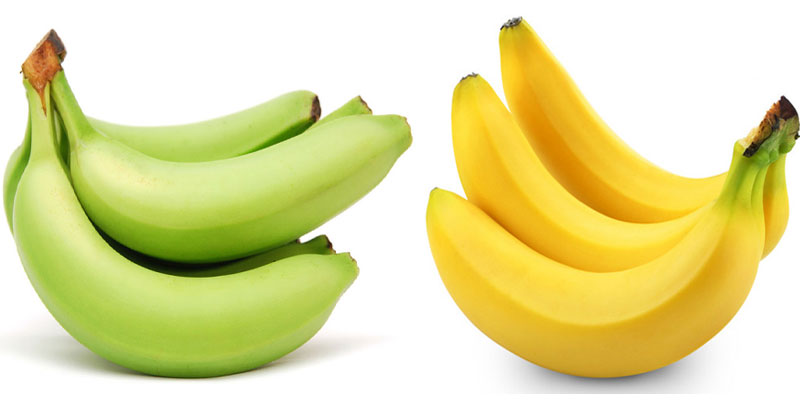
\includegraphics[width=8cm]{images/1_1.jpg}
% \caption{Nải chuối có thể màu lục hoặc màu vàng.}
% \end{wrapfigure}

\begin{wrapfigure}{l}{0.6\textwidth}
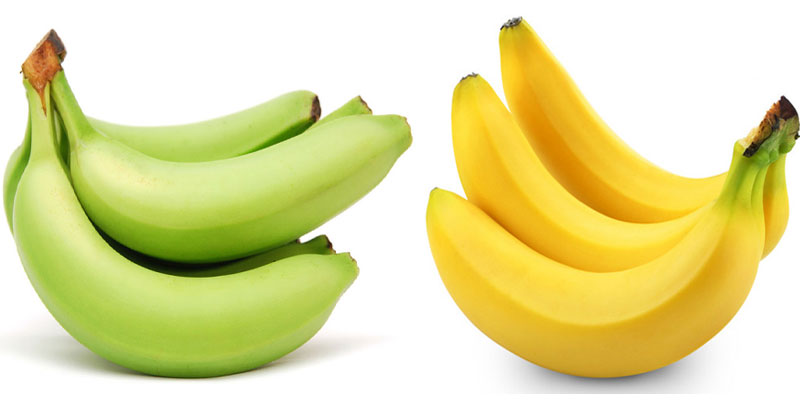
\includegraphics[width=8cm]{images/1_1.jpg} 
\caption{Nải chuối có thể màu lục hoặc màu vàng.}
\end{wrapfigure}

\noindent
Trước khi có sự xuất hiện của của ngành học sâu trong việc xử lý ảnh, đã có rất nhiều kỹ thuật được đưa ra cho quá trình tự động phục hồi màu cho ảnh xám. Nhưng để có được một kết quả ưng ý, đều hoặc nhiều hoặc ít dựa vào sự can thiệp của bàn tay con người. Sau khi học sâu bùng nổ trong ngành thị giác máy tính, rất nhiều mô hình học sâu ứng dụng mạng tích chập đã có thể học và tạo ra màu cho những ảnh xám.

\subsection{Mục tiêu}\label{objective}
Đồ án được đưa ra với mục đích xây dựng và huấn luyện một mô hình học sâu để tạo màu cho ảnh xám. Yêu cầu của màu tạo ra không cần thiết phải giống hoàn toàn so với màu thực, thay vào đó độ chân thực, hợp lí sẽ là thứ được hướng đến.\vspace{5pt}\\
Những nội dung chính được nghiên cứu, trình bày trong đồ án bao gồm:
\begin{itemize}
    \item Lựa chọn không gian màu thích hợp để sử dụng cho bài toán tạo màu.
    \item Mô hình học sâu để tạo màu - mạng đối nghịch tạo sinh với bộ kiến trúc mạng Unet.
    \item Xây dựng kiến trúc mạng Unet dựa vào xương sống mạng ResNet bằng học chuyển giao.
    \item Triển khai mô hình sử dụng ngôn ngữ lập trình Python.
\end{itemize}

%%%%%%%%%%%%%%%%%%%%%%%%%%%%%%%%%
\section{Lý thuyết}

\subsection{Không gian màu}
Hầu hết khi làm việc với ảnh số, ta sẽ thao tác với ảnh có không gian màu là \textbf{RGB}, tức ảnh có 3 kênh màu đỏ-lục-lam. Đây cũng là không gian màu phổ biến với đại đa số mọi người. Với ảnh thuộc không gian màu \textbf{RGB}, mỗi điểm ảnh sẽ có 3 giá trị \textbf{R-G-B}, mỗi giá trị nằm trong đoạn $[0, 255]$, tương ứng với 3 kênh màu để tạo nên được màu của chính điểm ảnh.

\begin{figure}[!h]
\captionsetup{width=0.8\textwidth}
\centering
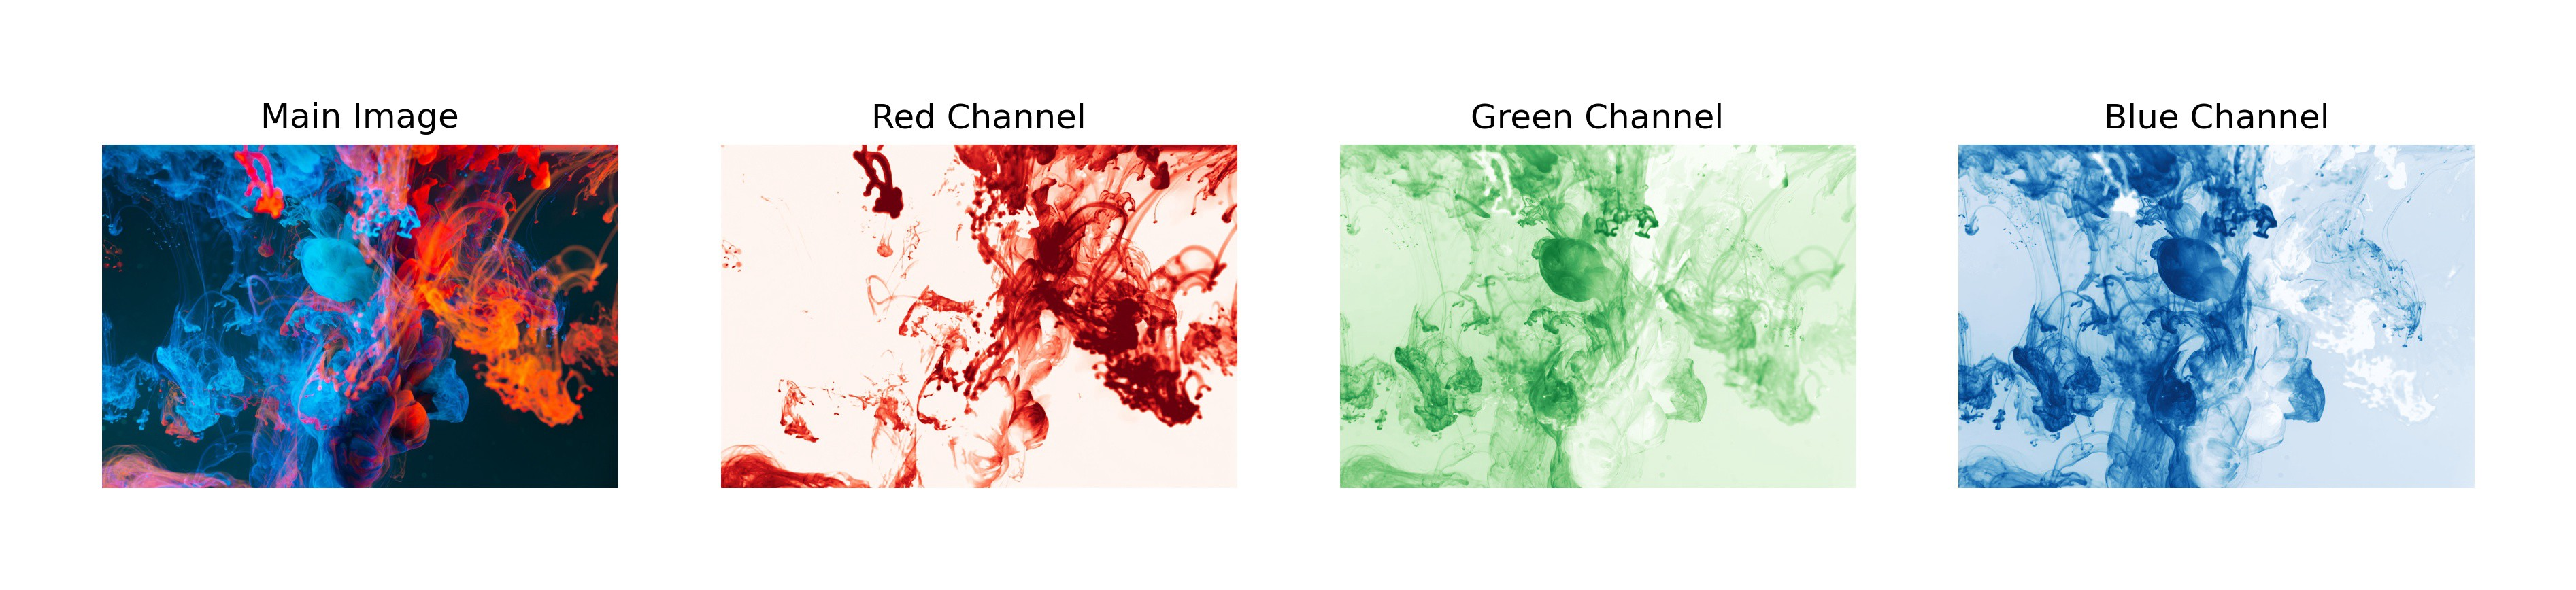
\includegraphics[width=16cm]{images/2_1.jpeg}
\caption{Các kênh màu đỏ, lục và lam được tách ra riêng biệt \cite{moeincolorization2020}.}
\label{fig:inspectrgb}
\end{figure}

\noindent
Ngoài RGB, một không gian màu khác cũng được sử dụng khá nhiều là không gian màu \textbf{L*a*b*}, không gian này cũng quan tấm đến 3 thông số của mỗi điểm ảnh. Thông số đầu tiên là \textbf{L*} đại diện cho độ sáng của của mỗi điểm ảnh. Giá trị \textbf{L*} càng lớn thì điểm ảnh càng nghiêng về màu trắng, ngược lại thì sẽ là màu đen. Hai thông số còn lại là \textbf{a*} và \textbf{b*} sẽ mang thông tin lần lượt là lục-đỏ và vàng-lam . Giá trị \textbf{a*} càng thấp thì điểm ảnh nghiên về lục nhiều, đỏ ít. Ngược lại thì lục ít, đỏ nhiều và tương tự với giá trị \textbf{b*}.

\begin{figure}[!h]
\captionsetup{width=0.8\textwidth}
\centering
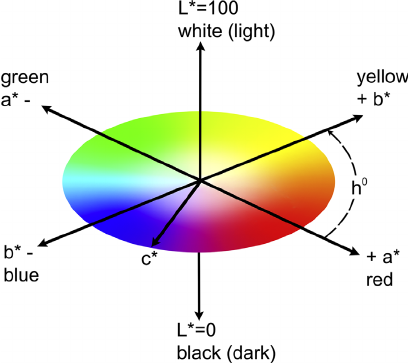
\includegraphics[width=8cm]{images/2_2.png}
\caption{Không gian màu Lab.}
\label{fig:labspace}
\end{figure}

\noindent
Khoảng giá trị của kênh \textbf{L*} nằm trong đoạn $[0, 100]$. Về phần 2 kênh còn lại là \textbf{a*} và \textbf{b*}, không có cụ thể một khoảng nhất định mà tuỳ thuộc vào phần mềm, chương trình mà ta sử dụng nhưng thông thường sẽ là đoạn $[-128, 127]$.\vspace{5pt}

\begin{figure}[!h]
\captionsetup{width=0.8\textwidth}
\centering
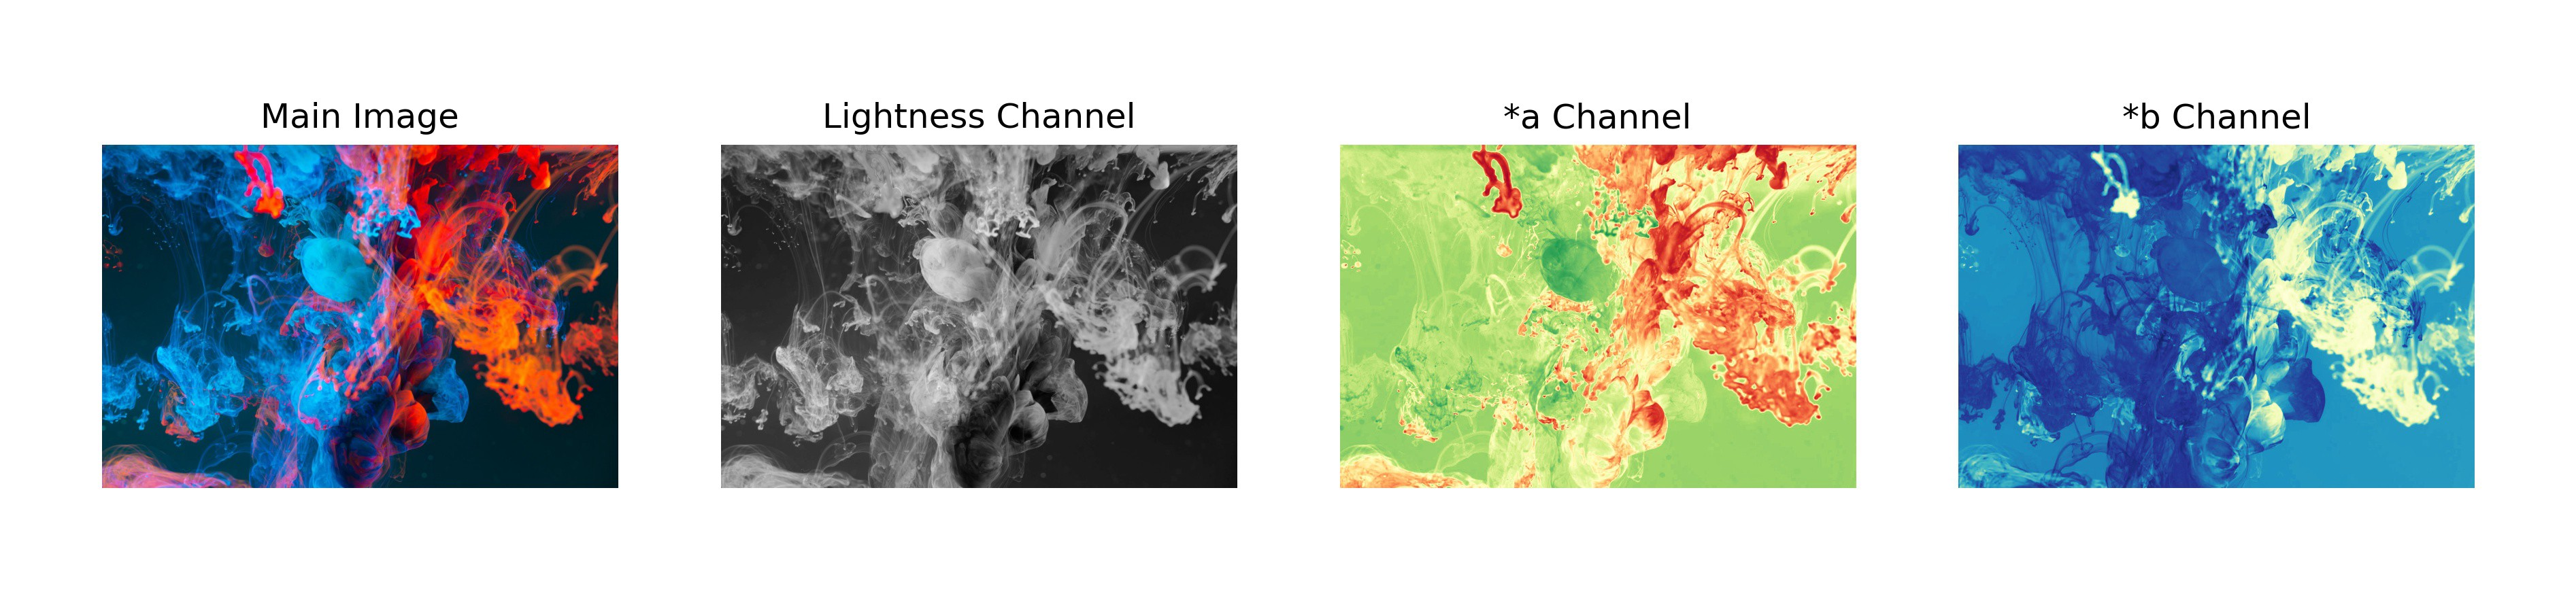
\includegraphics[width=16cm]{images/2_3.jpeg}
\caption{Các giá trị \textbf{L}, \textbf{a} và \textbf{b} được tách ra riêng biệt \cite{moeincolorization2020}.}
\label{fig:inspectlab}
\end{figure}

\noindent
Giữa hai không gian màu trên, mặc dù \textbf{RGB} có sự phổ biến nhiều hơn, nó vẫn không được lựa chọn để xử lý cho bài toán tạo màu. Sẽ có hai lợi thế khi sử dụng \textbf{L*a*b*} thay vì \textbf{RGB} \cite{wikilab2021}:
\begin{enumerate}[i)]
    \item Không gian màu \textbf{L*a*b*} được thiết kế để đồng nhất về cảm giác, điều này làm cho không gian màu này trở nên lý tưởng cho việc xử lí máy tính.
    \item Tận dụng kênh mức xám đầu vào để làm kênh độ sáng \textbf{L*} bằng cách điều chỉnh tỉ lệ. Khi đó mô hình chỉ phải dự đoán 2 kênh \textbf{a*} và \textbf{b*} thay vì phải dự đoán 3 kênh trong không gian \textbf{RGB}.
\end{enumerate}

\subsection{Những phương pháp được đề xuất}
Trong khoảng hai thập kỉ vừa qua, rất nhiều phương pháp đã được đề xuất. Chúng có thể được chia ra làm 3 loại phương pháp: Dựa vào những màu ban được đánh dấu ban đầu, dựa vào mẫu và cuối cùng là dùng học sâu. Hai loại phương pháp đầu tiên chưa phải là một phương pháp hoàn toàn tự động mà vẫn phải cần có sự can thiệp từ con người. Phương pháp thứ 3 là sử dụng học sâu là hoàn toàn tự động khi mô hình học sâu có thể học được màu tương ứng của các đối tượng từ những dữ liệu huấn luyện.\vspace{5pt}\\
Cách làm đơn giản nhất trong phương pháp \textbf{dựa vào những màu được đánh dấu ban đầu} có thể kể đén là \textbf{đánh dấu màu một vài điểm ảnh và dùng thuật toán loang}, được đề xuất bởi Levin \cite{alevincolorization}. Từ một tấm ảnh xám đầu vào, ta sẽ vẽ một vài màu cơ bản từ đó làm nền tảng, định hướng cho mô hình. Ý tưởng này xuất phát từ quan sát rằng, những điểm ảnh có độ sáng gần bằng nhau (mức xám xấp xỉ) và có khoảng cách trên ảnh gần nhau sẽ có khả năng tương tự cao dẫn đến màu giống nhau.\\
Một vài cách cải thiện độ hiệu quả của phương pháp trên như là sử dụng thông tin các cạnh để thuật toán loang hoạt động chính xác hơn \cite{huangcolorization}. Hay theo như Luan \cite{luancolorization}, ta đánh dấu mỗi màu cho mỗi phân đoạn khác nhau. 

\begin{figure}[!h]
\captionsetup{width=0.8\textwidth}
\centering
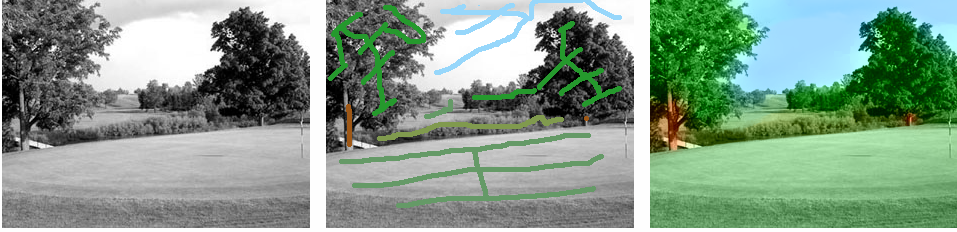
\includegraphics[width=15cm]{images/2_4.png}
\caption{Mô tả ý tưởng thuật toán đánh dấu vài điểm ảnh \cite{trungcolorization2018}.}
\label{fig:scribblemethod}
\end{figure}

\noindent
Những phương pháp thuộc loại phương pháp trên nhìn chung có kết quả màu rất tốt, nhưng lại đòi hỏi không ít sức người. Đặc biệt với những ảnh nhiều chi tiết thì việc đánh dấu màu sẽ trở nên khó khăn và tốn nhiều thời gian. Thêm nữa, việc chọn màu để đánh dấu cũng không phải là một vấn đề dễ dàng với một người có ít kinh nghiệm về màu sắc.\vspace{5pt}\\
\textbf{Dựa vào mẫu} là một loại phương pháp sử dụng một mẫu giống hoặc tương tự để giải quyết trọn vẹn bài toán. Với bài toán tô màu, phương pháp được khởi xướng bởi Welsh \cite{welshcolorization} sẽ \textbf{dựa vào màu của ảnh có bố cục tương tự}. Ta chọn ra một tấm ảnh mẫu có bố cục tương tự rồi dựa vào màu của ảnh mẫu, kết hợp chỉnh sửa để đưa ra dự đoán. Một vấn đề gặp phải khi ta sử dụng phương pháp trên đó là sự gắn kết không gian đã gần như bị bỏ qua. Để khắc phục, Ironi \cite{ironicolorization} đề xuất việc đưa màu của những phân đoạn của ảnh mẫu sang để dùng để đánh dấu màu rồi dùng thuật toán loang. Một hướng khác, Tai \cite{taicolorization} xây dựng xác suất từng phân đoạn của cả hai bức hình, sau đó chuyển màu từ ảnh mẫu sang ảnh cần tạo màu theo những vùng có kết quả thống kê gần tương xứng.

\begin{figure}[!h]
\captionsetup{width=0.8\textwidth}
\centering
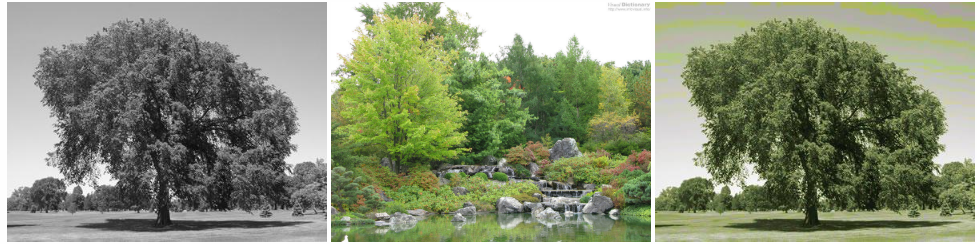
\includegraphics[width=15cm]{images/2_5.png}
\caption{Mô tả ý tưởng thuật toán ảnh có bố cục tương tự \cite{trungcolorization2018}.}
\label{fig:examplarmethod}
\end{figure}

\noindent
Dù loại phương pháp này đã giảm thiểu được phần nhiều tính thủ công, nhưng lại bị phụ thuộc lớn vào ảnh mẫu, ảnh mà phải có bố cục tương tự so với ảnh cần xử lý.\vspace{5pt}\\
Sau này, bằng cách tận dụng những cặp ảnh xám/màu, rất nhiều phương pháp \textbf{dựa vào học sâu} đã được ra đời. Đầu tiên nhất là Cheng \cite{chengcolorization}, khi triển khai một mô hình mạng nơ-ron sâu hoàn toàn tự động tạo màu thông qua việc xây dựng và tối ưu bài toán bình phương tối thiểu, với đầu vào của mô hình là bộ những mô tả ngữ cảnh. Nổi tiếng nhất trong phương pháp loại này có thể nói đến là Zhang \cite{zhangcolorization}, bằng việc học phân bố màu của mỗi điểm ảnh. Mô hình của Zhang được huấn luyện với đa thức entropy chéo kết hợp việc cân bằng các lớp hiếm để tạo ra được những màu ít xuất hiện.\vspace{5pt}\\
Những phương pháp học sâu đời đầu như Cheng có thể cải tiến dựa vào những nghiên cứu về mạng tích chập. Về sau, khi tập dữ liệu để huấn luyện trở nên lớn thì những mô hình học sâu gần như đã có thể tự động tô màu một cách cực kì chân thật, không thua gì so với kết quả được làm thủ công bởi những người thợ chỉnh sửa ảnh lâu năm, và có thể đánh lừa mắt người xem giữa ảnh gốc và ảnh được tô màu.\vspace{5pt}\\
Đồ án này ứng dụng khung mô hình mạng học sâu \textbf{pix2pix} \cite{isola2018imagetoimage} được đề xuất bởi Isola, một mô hình sử dụng mạng \textbf{GAN} \cite{goodfellow2014generative} có điều kiện với bộ sinh có kiến trúc mạng \textbf{Unet} \cite{ronneberger2015unet} kết hợp với bộ phân biệt Patch. Vì thế, để có thể có cái nhìn rõ ràng về kiến trúc mô hình được áp dụng xử lí bài toán tạo màu, ta cần sẽ đi qua những thành phần mạng chính tạo nên mô hình là GAN và Unet.

\subsection{Mạng đối nghịch tạo sinh (GAN - Generative Adversarial Network)}
Mạng GAN thuộc nhóm mô hình sinh dữ liệu mới. Dữ liệu sinh ra nhìn như thật nhưng không phải thật. Ví dụ như ảnh mặt người (xem hình \ref{fig:facesstylegan}) là do GAN sinh ra, không phải mặt người thật.

\begin{figure}[!h]
\captionsetup{width=0.8\textwidth}
\centering
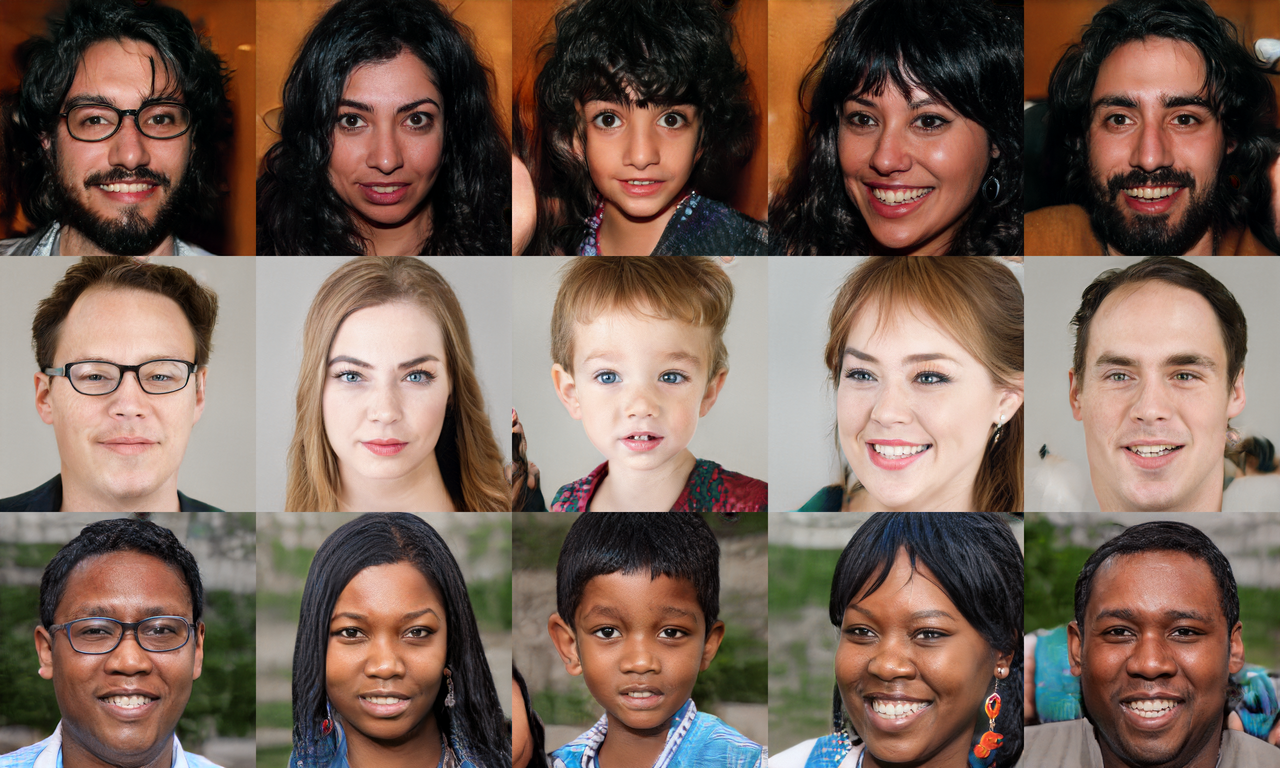
\includegraphics[width=14cm]{images/2_6.PNG}
\caption{Ảnh mặt người sinh ra bởi StyleGAN \cite{karras2019stylebased}.}
\label{fig:facesstylegan}
\end{figure}

\noindent
G - \textbf{G}enerative ý chỉ sinh, N - \textbf{N}etwork là mạng, còn A - \textbf{A}dversarial là đối nghịch. Lí do đối nghịch là trong mạng này được tạo nên từ sự kết hợp giữa 2 mạng là \textbf{bộ sinh} ($G$ \textit{- \textbf{G}enerator}) và \textbf{bộ phân biệt} (\textit{D - \textbf{D}iscriminator}), luôn luôn đối nghịch nhau trong quá trình huấn luyện. Trong khi bộ sinh cố gắng sinh ra các dữ liệu giống như thật thì bộ phân biệt lại cố gắng phân biệt đâu là dữ liệu được sinh ra từ bộ sinh và đâu là dữ liệu thật.\vspace{5pt}\\
Giả sử như bài toán đưa cho GAN là sinh ra tiền giả giống như tiền thật để có thể dùng được, thì bộ sinh là người làm tiền giả, còn bộ phân biệt giống như cảnh sát. Người làm tiền giả sẽ cố gắng làm ra những tờ tiền giả làm sao để cảnh sát không biết đó là giả, còn cảnh sát thì cố gắng học để phân biệt được tiền nào là giả, tiền nào là thật.\vspace{5pt}\\
Mục tiêu cuối cùng của GAN là người làm tiền giả phải có khả năng làm tiền giả sao cho cảnh sát không phân biệt được đâu là thật đâu là giả (50/50) để đem tiền giả đi tiêu thụ. Trong quá trình huấn luyện mạng GAN thì nhiệm vụ của cảnh sát là học cách phân biệt tiền giả và tiền thật, bên cạnh đó là nói cho người làm tiền giả là nên làm giả như thế nào cho giống thật hơn. Dần dần thì người làm tiền giả sẽ làm ra được tiền giống tiền thật và cảnh sát cũng trở nên thành thạo trong việc phân biệt tiền thật hay giả.

\begin{figure}[!h]
\captionsetup{width=0.8\textwidth}
\centering
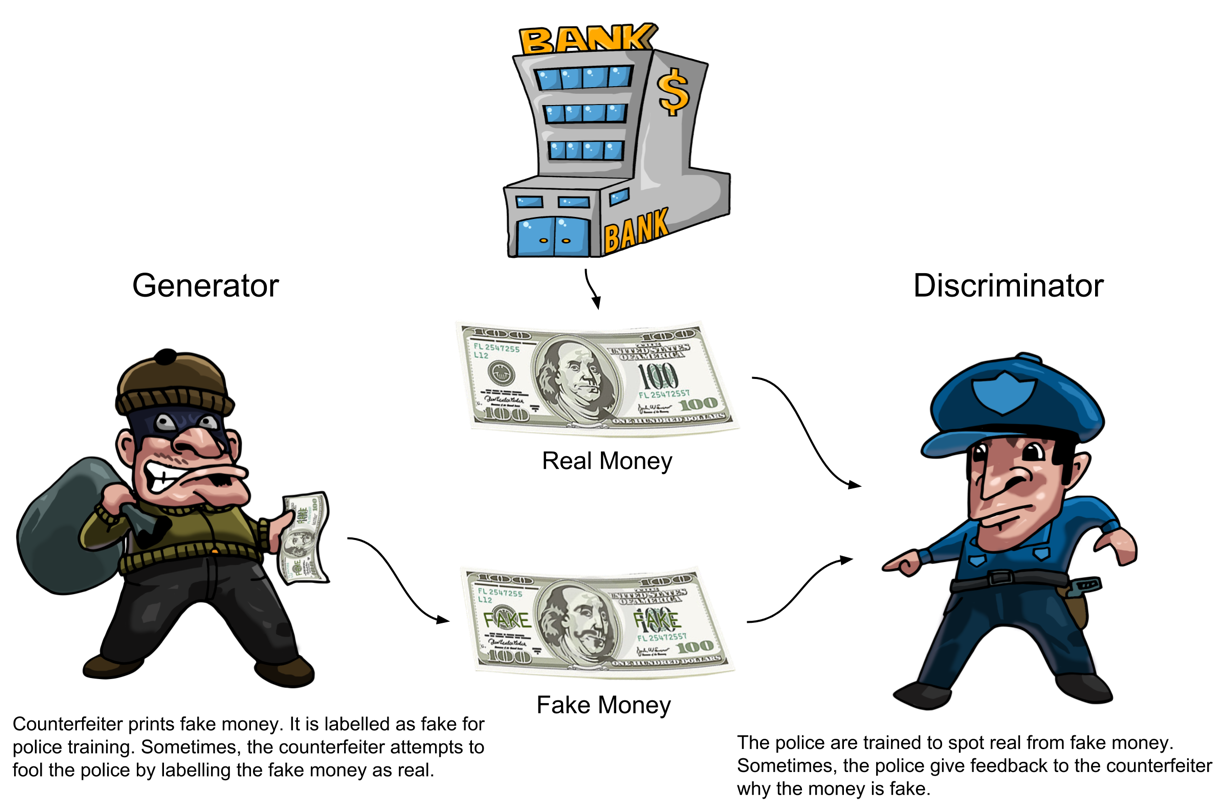
\includegraphics[width=12cm]{images/2_7.png}
\caption{Minh hoạ bộ sinh và bộ phân biệt trong mạng GAN \cite{richardgan2018}.}
\end{figure}

\noindent
Ý tưởng của GAN bắt nguồn từ \href{https://cs.stanford.edu/people/eroberts/courses/soco/projects/1998-99/game-theory/nonzero.html}{Non-Zero-Sum Games}\footnote{Stanford, \lq Non-Zero-Sum Games\rq, \href{https://stanford.io/3nCiLKq}{https://stanford.io/3nCiLKq}}, là một trò chơi đối kháng giữa 2 người, nếu một trong hai người thắng, thì người còn lại sẽ thua. Ở mỗi lượt, thì cả 2 đều muốn tối đa hoá cơ hội thắng của mình và tối thiểu hoá cơ hội thắng của đối phương. Trong lý thuyết trò chơi thì mô hình sẽ hội tụ khi cả bộ sinh và bộ phân biệt đạt tới trạng thái cân bằng Nash\footnote{Jørgen Veisdal, \lq The Nash equilibrium, explained\rq, \href{https://bit.ly/3ea57Lr}{https://bit.ly/3ea57Lr}}, tức là các bước tiếp theo của bất cứ ai trong hai người đều không làm thay đổi cơ hội thẳng của ai cả.\vspace{5pt}\\
Nhìn theo khía cạnh kỹ thuật, một bộ sinh sẽ sinh ra dữ liệu tốt (dữ liệu mà chúng ta mong muốn) nếu ta không thể chỉ ra đâu là dữ liệu giả và đâu là dữ liệu thật. Trong thống kê, điều này được gọi là bài kiểm tra từ hai tập mẫu - một bài kiểm tra để trả lời câu hỏi liệu tập dữ liệu $X = \{x_1, x_2, \dots, x_n\}$ và $X'=\{x_1', x_2', \dots, x_n'\}$ có được rút ra từ cùng một phân phối hay không. Sự khác biệt chính giữa hầu hết những bài nghiên cứu thông kê và GAN là GAN sử dụng ý tưởng này theo kiểu có tính xây dựng. Nói cách khác, thay vì chỉ huấn luyện mô hình để nói ``này, hai tập dữ liệu đó có vẻ như không đến từ cùng một phân phối'', thì GAN sử dụng phương pháp \textbf{kiểm tra trên hai tập mẫu}\footnote{Wikipedia, \lq Two-sample hypothesis testing\rq, \href{https://bit.ly/3vmFwVD}{https://bit.ly/3vmFwVD}} để cung cấp tín hiệu cho việc huấn luyện cho bộ sinh. Điều này cho phép ta cải thiện bộ sinh để có thể sinh dữ liệu tới khi ra được thứ gì đó giống như dữ liệu thực. Ở mức tối thiểu nhất, nó cần phải lừa được bộ phân biệt, kể cả bộ phân biệt của ta là một mạng nơ-ron sâu tân tiên nhất.

\begin{figure}[!h]
\captionsetup{width=0.8\textwidth}
\centering
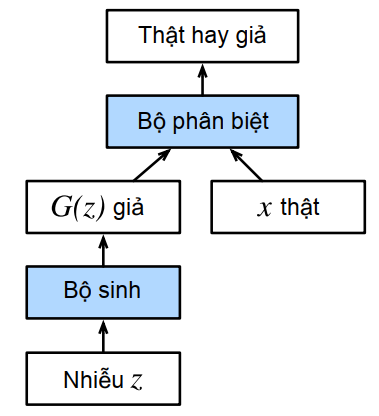
\includegraphics[width=7cm]{images/2_71.PNG}
\caption{Kiến trúc mạng đối nghịch tạo sinh.}
\end{figure}

\noindent
Bộ phân biệt là một bộ phân loại nhị phân nhằm phân biệt đầu vào $\mathbf{x}$ là thật (từ dữ liệu thật) hoặc giả (từ bộ sinh), được học theo kiểu giám sát. Đầu ra của bộ phân biệt là một số vô hướng $o \in \mathbb{R}$ dự đoán cho đầu vào $\mathbf{x}$, và sẽ được đưa qua hàm sigmoid $S(x) = 1/(1+e^{-x}), R = (0, 1)$ để nhận được xác suất dự đoán với giá trị càng gần 1 thì bộ phân biệt càng có xu hướng quyết định đó là dữ liệu thật. Hàm mất mát của bộ phân biệt cũng vì thế mà có dạng entropy chéo, nghĩa là:
\begin{align*}
    \min_{D}\left\{-y\log D\left(\mathbf{x}\right) - \left(1-y\right)\log\left(1-D\left(\mathbf{x}\right)\right)\right\}
\end{align*}
Còn đối với bộ sinh, sẽ được học theo kiểu không giám sát. Trước tiên nó cần được cho vài tham số ngẫu nhiên được xem là nhiễu $\mathbf{z} \in \mathbb{R}^d$ (\textbf{số chiều $d$ thường là 100}\footnote{Reddit, ``Why is Z-dimension for GANs usually 100?'', \href{https://bit.ly/33nXNpk}{https://bit.ly/33nXNpk}}) từ một nguồn, ví dụ phân phối chuẩn $\mathbf{z} \sim \mathcal{N}\left(\mu, \sigma^2\right)=\mathcal{N}\left(0, 1\right)$. Mục tiêu của bộ sinh là đánh lựa bộ phân biệt để phân loại $\mathbf{x'} = G\left(\mathbf{z}\right)$ là dữ liệu thật, nghĩa là, ta muốn $D\left(G\left(\mathbf{z}\right)\right) \approx 1$. Nói cách khác, cho trước một bộ phân biệt $D$, ta sẽ cập nhật tham số của bộ sinh $G$ nhằm cực đại hoá mất mát entropy chéo khi $y=0$, tức là:
\begin{align*}
    \max_G\left\{-\log\left(1-D\left(G\left(\mathbf{z}\right)\right)\right)\right\}
\end{align*}
Tóm lại, $D$ và $G$ đang chơi trò ``cực tiểu hoá cực đại'' với một hàm mục tiêu như sau:
\begin{align*}
    \min_D\max_G\left\{-\mathbb{E}_{\mathbf{x}\sim \text{data}}\log D\left(\mathbf{x}\right)-\mathbb{E}_{\mathbf{z} \sim \text{noise}}\log\left(1-D\left(G\left(\mathbf{z}\right)\right)\right)\right\}\\
    \Leftrightarrow \min_G\max_D\left\{\mathbb{E}_{\mathbf{x}\sim \text{data}}\log D\left(\mathbf{x}\right)+\mathbb{E}_{\mathbf{z} \sim \text{noise}}\log\left(1-D\left(G\left(\mathbf{z}\right)\right)\right)\right\}
\end{align*}
Kí hiệu $\mathbb{E}$ ở đây chính là kì vọng toán, tương đương việc lấy trung bình của tất cả dữ liệu.

\begin{figure}[!h]
\captionsetup{width=0.8\textwidth}
\centering
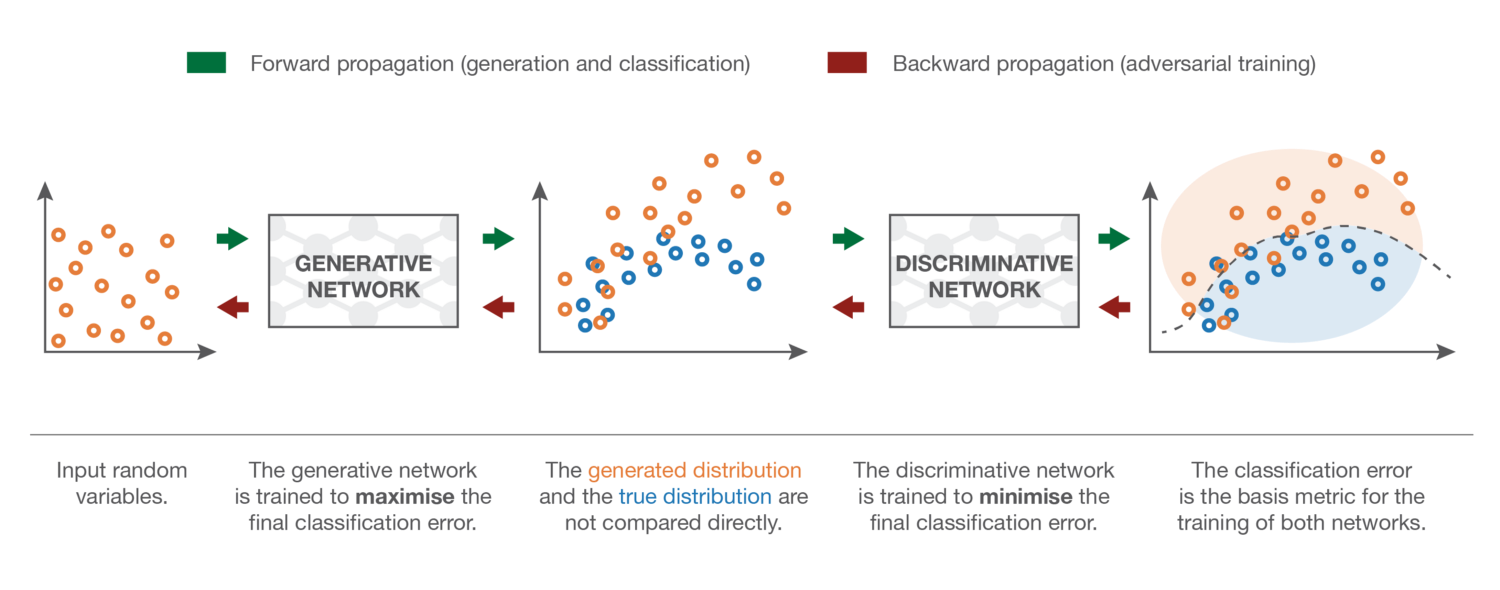
\includegraphics[width=16.5cm]{images/2_72.png}
\caption{Mô phỏng quá trình huấn luyện mạng GAN \cite{josephgan2019}.}
\label{fig:forandbackgan}
\end{figure}

\noindent
Quá trình huấn luyện mạng GAN cũng không khác gì so với những mạng học sâu khác là bao. Như được mô tả trong hình 2.9, quá trình được bắt đầu bằng việc lan truyền thuận khi bộ sinh lấy một biến ngẫu nhiên $\mathbf{z}$ từ phân bố được chọn ban đầu rồi dựa vào đó sinh ra một biến ngẫu nhiên $G(\mathbf{z})$ thuộc một phân bố khác. Dữ liệu thật $\mathbf{x}$ hiển nhiên sẽ có phân bố khác với phân bố của $G(\mathbf{z})$. Bộ phân biệt sẽ có nhiệm vụ tạo ra đường biên thích hợp để phân biệt hai phân bố $G(\mathbf{z})$ và $\mathbf{x}$. Kết thúc quá trình lan truyền thuận là quá trình lan truyền ngược, bộ phân biệt được huấn luyện tốt hơn để phân biệt hai phân bố đồng thời giúp cho bộ sinh điều chỉnh để có thể sinh ra $G(\mathbf{z})$ có phân bố giống với lại phân bố của $\mathbf{x}$. Ta chỉ điều chỉnh lại phân bố của $G(\mathbf{z})$ chứ không điều chỉnh phân bố của $\mathbf{z}$ vì không cần thiết và phức tạp.

\subsection{Mạng Unet}
Unet là một kiến trúc được phát triển nhằm phân vùng các cấu trúc nơ-ron thần kinh trong não người. Kiến trúc này lần đầu được áp dụng đã giành chiến thắng trong cuộc thi EM segmentation challenge at ISBI 2012.\footnote{ISBS Challenge: Segmentation of neuonal structures in EM stacks, \href{https://bit.ly/2RAIyqR}{https://bit.ly/2RAIyqR}}

\noindent
Mạng Unet bao gồm 2 nhánh đối xứng nhau hình chữ U nên được gọi là Unet. Kiến trúc mạng bao gồm 2 phần là \textbf{thu hẹp} ở nhánh trái và \textbf{phần mở rộng} ở nhánh phải. Mỗi phần sẽ thực hiện một nhiệm vụ riêng như sau:

\begin{itemize}
    \item Phần thu hẹp: làm nhiệm vụ trích lọc đăc trưng để tìm ra bối cảnh của hình ảnh (\textit{WHAT}). Vai trò của phần thu hẹp tương tự như một bộ mã hoá. Một mạng tích chập sâu sẽ đóng vai trò trích lọc đặc trưng. Lý do nhánh được gọi là thu hẹp vì kích thước dài và rộng của các tầng giảm dần. Độ phân giải được giảm bằng cách sử dụng \textbf{gộp cực đại} hoặc dùng tích chập có \textbf{đệm} và \textbf{sải bước} hợp lí.
    
    \item Phần mở rộng: Gồm các tầng đối xứng tương ứng với các tầng của nhánh thu hẹp có vai trò như một bộ giải mã. Ở phần này, độ phân giải của các tầng được tăng lại để biết được vị trí (\textit{WHERE}) từ đó đánh dấu nhãn của từng điểm ảnh. Để làm được điều này, ta cần sử dụng kĩ thuật giải chập. Có nhiều phương pháp để giải chập, chẳng hạn như sao chép các giá trị điểm ảnh liền kề theo các kích thước cửa sở hoặc một phương thức khác là sử dụng \textbf{tích chập giãn nở}. Nhưng được áp dụng nhiều nhất là \textbf{tích chập chuyển vị} cùng với đêm và sải bước thích hợp.
\end{itemize}

\begin{figure}[!h]
\captionsetup{width=0.8\textwidth}
\centering
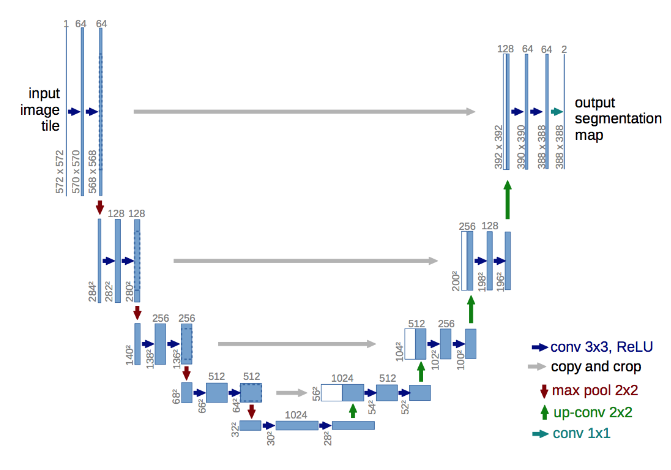
\includegraphics[width=15cm]{images/2_8.png}
\caption{Kiến trúc mô hình mạng Unet \cite{ronneberger2015unet}.}
\end{figure}

\noindent
Đặc trưng riêng trong cấu trúc của Unet đó là có những \textbf{kết nối tắt} đối xứng giữa các tầng của nhánh bên trái tương ứng với các tầng bên nhánh bên phải. Việc kết nối tắt theo kiến trúc Unet là một điểm mới so với kiến trúc mã hoá và giải mã thông thường nhằm bổ sung thêm thông tin và gia tăng độ chính xác. Chi tiết về kết nối tắt, có thể tham khảo một số mạng tích chập hiện đại sử dụng như phương pháp trên \cite{he2015deep}, \cite{huang2018densely}. Ngoài ra kết nối tắt còn khắc phục hiện tượng gradient biến mất \cite{adaloglou2020skip}.

\subsection{Kiến trúc được áp dụng}
Bài toán tạo màu có thể được tóm tắt như sau:
\begin{tcolorbox}
Cho một ảnh đầu vào có kích thước $S\times S = 256\times 256$ chỉ có thông tin cường độ mức sáng mỗi điểm ảnh là $\mathbf{L^*} \in \mathbb{R}$, ta cần phải xây dựng một ánh xạ $\mathcal{G}: \mathbf{L^*} \rightarrow \left(\mathbf{a^*}, \mathbf{b^*}\right) \in \mathbb{R}^2$ sao cho $\mathcal{I} = \left\{p_{ij} = \left(\mathbf{L^*}_{ij}, \mathbf{a^*}_{ij}, \mathbf{b^*}_{ij}\right)\vert p_{ij} \text{ là điểm ảnh ở hàng } i \text{, cột } j\right\}$ là một ảnh màu hợp lí, chân thực với $\mathbf{a^*}$ và $\mathbf{b^*}$ lần lượt là 2 kênh màu lục-đỏ và vàng-lam trong không gian màu \textbf{L*a*b*}.
\end{tcolorbox}
\noindent
Trong mạng GAN được huấn luyện, bộ sinh $G$ sẽ sinh ra 2 kênh màu \textbf{a*} và \textbf{b*} - Chính là ánh xạ $\mathcal{G}$ cần tìm. Còn bộ phân biệt $D$ có nhiệm vụ phân biệt ảnh màu đưa vào là thật hay giả.

\begin{figure}[!h]
\captionsetup{width=0.8\textwidth}
\centering
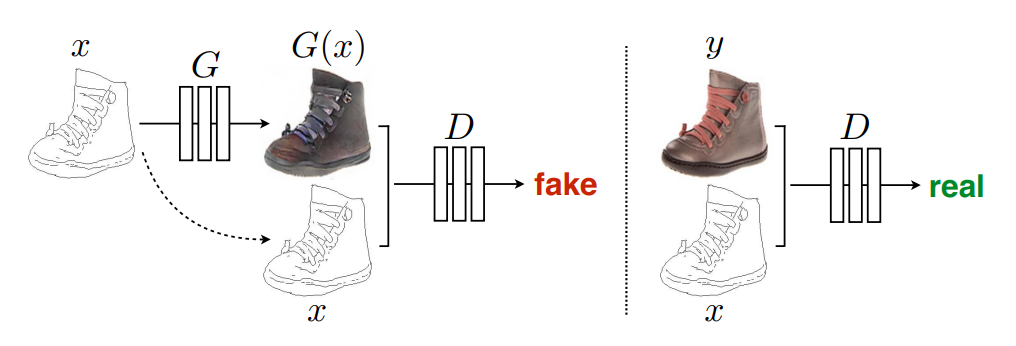
\includegraphics[width=14cm]{images/2_9.PNG}
\caption{Mô hình GAN dự đoán ảnh dựa vào đường viền. Một bài toán tương tự với bài toán tạo màu cho ảnh \cite{isola2018imagetoimage}.}
\end{figure}

\noindent
Bộ sinh theo kiến trúc mạng Unet với đầu vào là một ảnh chỉ có một kênh biểu thị cho cường độ sáng mỗi điểm ảnh là $\mathbf{X} \in \mathbb{R}^{S\times S \times 1}$. Bức ảnh sẽ được truyền vào một kiến trúc mạng tích chập để trích lọc đặc trưng thông qua quá trình mã hoá. Ở quá trình này, kích thước đầu ra ở mỗi tầng sẽ giảm dần theo bội 2. Trong giai đoạn giải mã, các đặc trưng được kết hợp với phía trái nhánh chữ U là phần mã hoá để biến đổi lại thành ảnh đích bằng tích chập chuyển vị, và mỗi tầng sẽ có kích thước tăng dần cũng theo bội 2. Kết quả trả ra sau cùng là hai kênh màu $\mathbf{\widehat{Y}} \in \mathbb{R}^{S\times S \times 2}$. Khi đó, ảnh giả được bộ sinh tạo ra là:
\begin{align*}
    \widehat{\mathcal{I}} = \left\{p_{ij} = \left(\mathbf{L^*}_{ij}, \widehat{\mathbf{a^*}}_{ij}, \widehat{\mathbf{b^*}}_{ij}\right) \vert \mathbf{L^*}_{ij} \in \mathbf{X}, \left(\widehat{\mathbf{a^*}}_{ij}, \widehat{\mathbf{b^*}}_{ij}\right) \in \mathbf{\widehat{Y}}\right\}
\end{align*}
\noindent
Đầu vào của bộ phân biệt là ảnh $\mathcal{I} = \left(\mathbf{X}, \mathbf{Y}\right) \in \mathbb{R}^{S \times S \times 3}$ hoặc ảnh $\widehat{\mathcal{I}} = \left(\mathbf{X}, \mathbf{\widehat{Y}}\right) \in \mathbb{R}^{S \times S \times 3}$. Các ảnh sẽ có nhãn đầu ra là thật nếu cặp dữ liệu đầu vào có $\mathbf{Y}$ được lấy từ tập huấn luyện và trái lại là khi dữ liệu đầu vào có $\mathbf{\widehat{Y}}$ được sinh ra từ bộ sinh thì sẽ mang nhãn giả. Một điểm khác biệt dễ thấy so với bộ phân biệt ở mang GAN thông thường là thay vì chỉ nhận được đầu vào là $\mathbf{Y}$ hoặc $\mathbf{\widehat{Y}}$ cho việc phân loại mà còn kèm theo $\mathbf{X}$. Đây chính là điều kiện ràng buộc cho quyết định của bộ sinh, vì muốn biết màu thật hay giả thì phải biết màu đó của thứ gì.\vspace{5pt}\\
Hàm mất mát của mô hình GAN của chúng ta cũng không quá khác biệt so với hàm mất mát của một mạng GAN thông thường, cụ thể là:
\begin{align*}
    \mathcal{L}_{cGAN}(G, D) = \mathbb{E}_{\mathbf{X}, \mathbf{Y}}\log D\left(\mathbf{X}, \mathbf{Y}\right) + \mathbb{E}_{\mathbf{X}}\log \left(1 - D\left(\mathbf{X}, G\left(\mathbf{X}\right)\right)\right)
\end{align*}
\noindent
Nhiễu $\mathbf{z}$ không được đề cập trong công thức hàm mất mát ở đây, tuy nhiên trong \cite{isola2018imagetoimage} vẫn được xuất hiện. Các tác giả đã cố gắng tạo ra nhiễu từ việc sử dụng kỹ thuật \textbf{dropout} trong giai đoạn huấn luyện và cả thử nghiệm. Nếu ta không dùng kỹ thuật dropout, mô hình vẫn sẽ có thể được huấn luyện và đưa ra kết quả dự đoán tốt tuy nhiên không được tổng quát, kết quả dự đoán của mô hình sẽ khá bị bó buộc khi phân phối sẽ chỉ có thể là hàm delta. Nhưng theo như trả lời của tác giả \cite{replyrandomnoisez}, mô hình không thực sự cần đến nhiễu nếu đầu vào đủ phức tạp. Lúc đó đầu vào đóng vài trò như nhiễu. Và với bài toán tô màu, đầu vào là một bức ảnh xám được đánh giá là đủ phức tạp nên thành phần nhiễu được phép bỏ qua.\vspace{5pt}\\
Trong \cite{isola2018imagetoimage} cũng chỉ ra rằng, bằng việc kết hợp giữa hàm mất mát của GAN với một hàm mất mát truyền thống như chuẩn bậc 1 hoặc chuẩn bậc 2 cho bộ sinh thì khi đó, ngoài việc đánh lừa được bộ phân biệt thì nó còn phải làm sao sinh ảnh giống với kết quả có thực trong dữ liệu huấn luyện thông qua tối thiểu hoá chuẩn bậc 1 hoặc chuẩn bậc 2. Bên dưới là thành phần chuẩn bậc 1 được lựa chọn để giải quyết bài toán tạo màu:
\begin{align*}
    \mathcal{L}_{L1}(G) = \mathbb{E}_{\mathbf{X}, \mathbf{Y}}\left|\left|\mathbf{Y} - G(\mathbf{X})\right|\right|_1
\end{align*}
Lí do để chọn chuẩn bậc 1 thay vì chuẩn bậc 2 có thể được lí giải một cách trực quan, là do chuẩn bậc 2 có xu hướng trừng phạt mất mát nhiều hơn so với chuẩn bậc 1, do đó điều này làm bó buộc kết quả dự đoán của bộ sinh khiến cho mô hình có xu thế bảo thủ, sẽ đưa dự đoán bằng cách lấy giá trị trung bình để tối thiểu sự trừng phạt. Thay vì vậy, chuẩn bậc 1 lại nhẹ nhàng trong việc trừng phạt hơn, khiến cho mô hình có thể sáng tạo để đưa ra dự đoán phiêu lưu hơn. Để hiểu hơn về việc lựa chọn chuẩn bậc 1 hay chuẩn bậc 2, có thể tham khảo \cite{replynorm1ornorm2}.\vspace{5pt}\\
Cuối cùng, mô hình ta cần phải tối ưu là:
\begin{align*}
    G^* = \arg\underset{G}{\min}\underset{D}{\max}\mathcal{L}_{cGAN}(G, D) + \lambda \mathcal{L}_{L1}(G)
\end{align*}
Trong đó, $\lambda$ là hệ số cân bằng để giúp cho sự chênh lệch giữa hai hàm mất mát không bị áp đảo nghiêng về một bên, khiến một hàm bị lu mờ trong quá trình huấn luyện.\\
Thông thường giá trị hàm mất mát của GAN sẽ có giá trị lớn hơn nhiều so với hàm chuẩn 1. Nên xu hướng chọn $\lambda$ sẽ là một số lớn hơn $1$, và thường giá trị được chọn sẽ là $\lambda = 100$.

\begin{figure}[!h]
\captionsetup{width=0.8\textwidth}
\centering
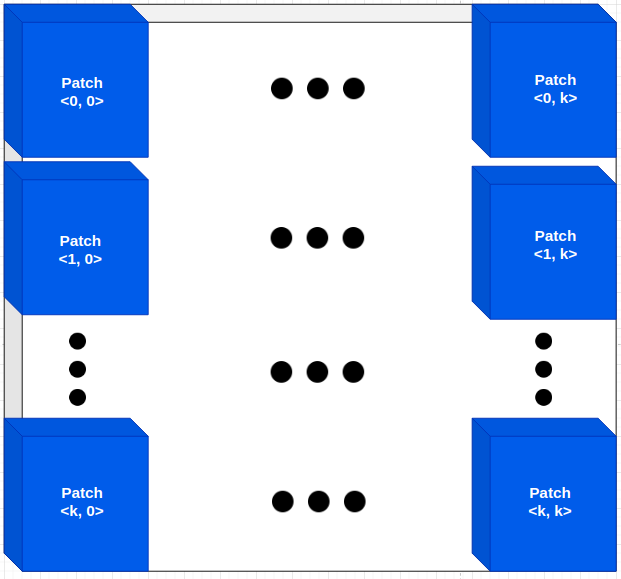
\includegraphics[width=8cm]{images/patch.png}
\caption{Hình ảnh giả sử được đầu vào chia thành $k\times k$ Patch \cite{khanhpix2pix2020}.}
\end{figure}

\noindent
Một điểm khác biệt nữa của bộ phân biệt trong mô hình này so với những bộ phân biệt trong các mô hình GAN thông thường là bộ phân biệt của chúng ta là làm việc theo Patch. Một bộ phân biệt thông thường chỉ trả về một số vô hướng thì bộ phân biệt Patch sẽ trả về một ma trận $\mathbf{P_D} \in \mathbb{R}^{k\times k}$ bằng cách phân loại từng vùng $N \times N$ của đầu vào là thật hay giả thay vì toàn bộ một lúc. Những vùng $N \times N$ này được gọi là vùng nhận thức và phân loại mỗi vùng nhận thức sẽ cho một giá trị $\left[\mathbf{P_D}\right]_{ij}$. Về bản chất, bộ phân biệt Patch vẫn là một kiến trúc mạng tích chập gồm nhiều tầng tích chập liên tiếp nhau, nhưng chúng ta không thực hiện làm phẳng ở gần cuối để truyền qua các lớp kết nối đầy đủ. Mà thay vào tính toán để ra được dự báo xác suất trên mỗi Patch rơi vào ảnh thật. Xác suất để toàn bộ đầu vào là thật sẽ là trung bình cộng của toàn bộ $k^2$ Patch. Cách tính như vậy sẽ mang lại hiệu quả nếu áp dụng trên các Patch có kích thước lớn vì có vùng nhận thức lớn hơn. Kết quả xác suất trung bình của nhiều Patch cũng sẽ chuẩn xác hơn. Sau khi đã thử qua một số kích thước Patch như $1\times 1, 16\times 16, 70\times 70, 286\times 286$ thì kích thước Patch tốt nhất theo \cite{isola2018imagetoimage} là $70 \times 70$.\vspace{5pt}\\
Kiến trúc các tầng của một bộ phân biệt Patch $70\times 70$ có thể biểu diễn đơn giản như sau:
\begin{align*}
    \text{I} \rightarrow \text{2C64} \rightarrow \text{2C128} \rightarrow \text{2C256} \rightarrow \text{1C512} \rightarrow \text{O}
\end{align*}
Với $\text{sCk}$ là một tầng tích chập gồm $k$ bộ lọc và có sải bước là $s$. Tầng cuối cùng $\text{O}$ sử dụng sải bước là $1$ và chỉ sử dụng duy nhất $1$ bộ lọc để trả ra ma trận $\mathbf{P_D}$ và kích hoạt hàm sigmoid để lấy xác suất. Tất cả các tầng đều sử dụng kích thước bộ lọc là $4$ cùng với kích thước đệm là $1$.

\begin{figure}[!h]
\captionsetup{width=0.8\textwidth}
\centering
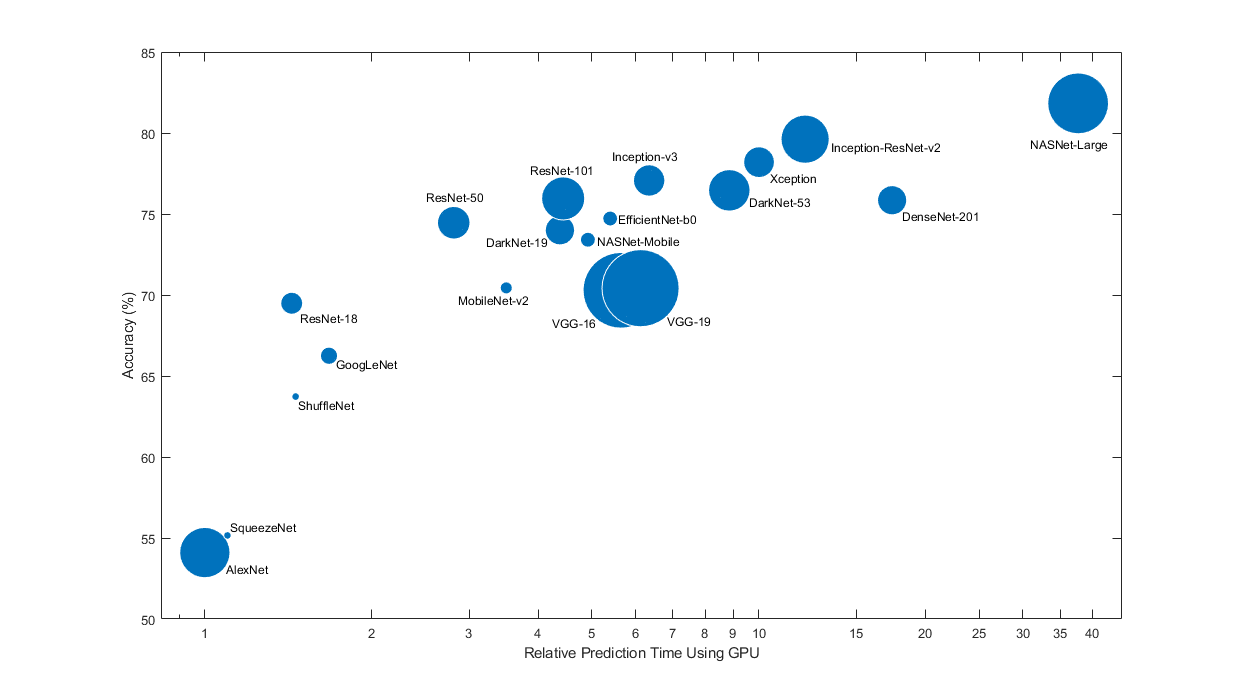
\includegraphics[width=10cm]{images/3_3.png}
\caption{Mô tả vùng nhận thức qua các tầng.}
\end{figure}

\noindent
Ta hoàn toàn có thể tính ngược lại được vùng nhận thức dựa vào thông tin kích thước bộ lọc và sải bước. Ta đã biết rằng, kích thước đầu ra sau khi qua một bộ lọc được tính bằng \cite{replycalcnnsize}:
\begin{align*}
    W_{\text{output}} = \left\lfloor\dfrac{W_{\text{input}} - K + 2P}{S}\right\rfloor + 1
\end{align*}
Như vậy, bằng các phép biến đổi ta suy ra được:
\begin{align*}
    W_{\text{input}} = K - 2P + S\left(W_{\text{output}} - 1\right)
\end{align*}
Tuy nhiên, khi suy ngược lại để tính vùng nhận thức ta cần quan tâm vùng ảnh không có đệm. Do đó công thức để tính kích thước vùng nhận thức $F$ từng tầng sẽ là:
\begin{align*}
    F_{\text{input}} = K + S\left(F_{\text{output}} - 1\right)
\end{align*}
Áp dụng công thức trên, ta sẽ tính được kích thước vùng nhận thức của mỗi giá trị đầu ra theo như kết quả sau đây:
\begin{align*}
    F_4 &= K + S_4(F_5 - 1) = 4 + 1(1-1) = 4\\
    F_3 &= K + S_3(F_4 - 1) = 4 + 1(4-1) = 7\\
    F_2 &= K + S_2(F_3 - 1) = 4 + 2(7-1) = 16\\
    F_1 &= K + S_1(F_2 - 1) = 4 + 2(16-1) = 34\\
    F_0 &= K + S_0(F_1 - 1) = 4 + 2(34 - 1) = 70
\end{align*}

\subsection{Học chuyển giao cho bộ sinh bằng xương sống ResNet18}\label{transferlearning}
Trong mạng cGAN của chúng ta, được quan tâm hơn cả là bộ sinh vì nó là ánh xạ $\mathcal{G}$ ta cần tìm để giải bài toán tạo màu. Kiến trúc bộ sinh được đề xuất trong \cite{isola2018imagetoimage} như sau:
\begin{align*}
    &\text{nhánh trái:} \text{I} \rightarrow \text{C64} \rightarrow \text{C128} \rightarrow \text{C256} \rightarrow \text{C512} \rightarrow \text{C512} \rightarrow \text{C512} \rightarrow \text{C512} \rightarrow \text{C512}\\
    &\text{nhánh phải:} \rightarrow \text{D512} \rightarrow \text{D1024} \rightarrow \text{D1024} \rightarrow \text{D1024} \rightarrow \text{D512} \rightarrow \text{D256} \rightarrow \text{D128} \rightarrow \text{D2}
\end{align*}
Trong đó, $\text{Ck}$ là một tầng tích chập $k$ bộ lọc, $\text{Dk}$ là một tầng giải chập bằng tích chập chuyển vị với $k$ bộ lọc. Cả 2 quá trình chập và giải chập đều sử dụng kích thước bộ lọc là $4$, sải bước $2$ và đệm $1$.\vspace{5pt}\\
Xây dựng mô hình theo kiến trúc trên không quá khó, nhưng huấn luyện để có được kết quả tốt tương tự, khi hạn chế về số lượng và chất lượng của tập dữ liệu, cũng như phần cứng máy tính bị giới là khá thử thách (xem phần \ref{badexperiment}).\vspace{5pt}\\
Cải thiện mô hình mà vẫn tiết kiệm chi phí, phương pháp học chuyển giao được áp dụng để làm điều này. Kiến trúc cho bộ sinh vẫn sẽ là kiến trúc theo mạng Unet, tuy nhiên sẽ được chuyển giao bằng cách lấy xương sống là ResNet18 \cite{christopherresunet2019}. Có 3 họ mạng được chủ yếu dùng để làm xương sống cho Unet là VGG, ResNet và Xception \cite{backboneresnet2020}. Trong những họ mạng trên, ResNet18 có kích thước không quá lớn \cite{Khan_2020}, phù hợp để huấn luyện với phần cứng bị giới hạn. Một lưu ý là mạng ResNet18 sẽ chỉ làm phía mã hoá, tức nhánh bên trái của chữ U chứ không hề xây dựng toàn bộ cả mạng Unet. Phần mã hoá sẽ được tự động khởi tạo bởi thư viện fastai\footnote{fastai Documentation, ``Dynamic UNet'', \href{https://docs.fast.ai/vision.models.unet.html}{https://docs.fast.ai/vision.models.unet.html}}.

%%%%%%%%%%%%%%%%%%%%%%%%%%%%%%%%%
\section{Triển khai mô hình}

\subsection{Ngôn ngữ lập trình \& Thư viện chính}
Ngôn ngữ lập trình được sử dụng để triển khai mô hình là \textbf{Python} với sự hỗ trợ chính của thư viện \textbf{PyTorch}. Để cài đặt những công cụ này, có thể theo đường dẫn bên dưới:
\begin{itemize}
    \item Python: \href{https://www.python.org/downloads/}{https://www.python.org/downloads/}
    \item PyTorch \href{https://pytorch.org/get-started/locally/}{https://pytorch.org/get-started/locally/}
\end{itemize}
Thư viện \textbf{fastai} (bản mới nhất) cũng được cài đặt cho việc xây dựng mạng Unet và một số tác vụ liên quan. Để cài đặt, mở cửa sổ dòng lệnh (đã được cài đặt môi trường Python) rồi thực thi mã lệnh:
\begin{lstlisting}
pip install fastai --upgrade
\end{lstlisting}

\noindent
Toàn bộ mã nguồn, cũng như những tệp liên quan trong quá trình hoàn thành mô hình, có thể tìm thấy trong thư mục đồ án tại:
\begin{itemize}
    \item Github: \href{https://github.com/dee-ex/EE3151\_SEM202\_PROJECT}{https://github.com/dee-ex/EE3151\_SEM202\_PROJECT}
\end{itemize}
Để có thể biết được đầy đủ những thư viện cũng như phiên bản thư viện được sử dụng, tham khảo tệp tin \texttt{requirements.txt} trong đường dẫn thư mục đồ án.

\subsection{Tập dữ liệu}
Tập dữ liệu được chọn sử dụng là tập \href{https://cocodataset.org/#download}{\textbf{COCO}} có trong thư viện \textbf{fastai}, ta có thể dễ dàng tải về. Sô lượng ảnh được chọn để huấn luyện là $10,000$. Tất cả đều được chọn ngẫu nhiên và có xáo trộn.

\begin{figure}[!h]
\captionsetup{width=0.8\textwidth}
\centering
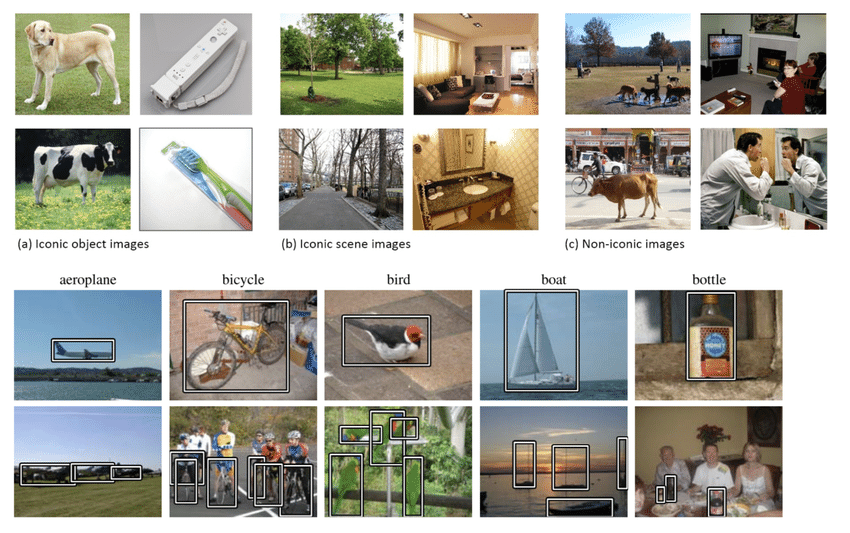
\includegraphics[width=15cm]{images/3_1.png}
\caption{Hình ảnh trích từ tập dữ liệu COCO.}
\end{figure}

\subsection{Chuẩn hoá và làm giàu dữ liệu}\label{normalization}

Chuẩn hoá dữ liệu đầu vào là bước tiền xử lí giúp tăng tốc độ hội huấn luyện cho mô hình, giảm sự phụ thuộc của gradient vào tỉ lệ các tham số và một số lợi ích khác \cite{jasonscaledata2019, benscaledata2012}. Ở đây, 3 kênh dữ liệu sẽ được chuẩn hoá cùng về một khoảng $[-1, 1]$:
\begin{align*}
    \mathbf{L^*}_{\text{normalization}} = \dfrac{\mathbf{L^*}}{50} - 1\\
    \mathbf{(a^*, b^*)}_{\text{normalization}} = \dfrac{\mathbf{(a^*, b^*)}}{110}
\end{align*}

\noindent
Bên cạnh đó, kích thước ảnh cũng sẽ được điều chỉnh lại thành ảnh vuông kích thước $256\times 256$ nếu cần thiết, và sử dụng lật đối xứng theo trục tung để làm giàu dữ liệu cho việc huấn luyện.

\subsection{Huấn luyện mô hình}
Cách thức huấn luyện mô hình sử dụng Python-PyTorch được tham khảo chính từ \cite{aladdinperssonyoutube, moeincolorization2020}, đồng thời cũng có thêm một vài tham khảo về việc sử dụng Keras \cite{tuannguyenpix2pix2020, khanhpix2pix2020, jasonpix2pix2019} để huấn luyện.\vspace{5pt}\\
Vì mô hình bộ sinh phức tạp hơn rất nhiều so với bộ phân biệt, vậy nên để cho quá trình huấn luyện GAN được ổn định hơn, ta sẽ tiền huấn luyện \cite{ham2020unbalanced} độc lập bộ sinh bằng $\mathcal{L}_{\text{L1}}(G)$ qua 20 epoch với kích thước batch là 16. Mỗi epoch mất khoảng 6--7 phút khi huấn luyện trên Google Colab\footnote{Google Colab, \href{https://colab.research.google.com/}{https://colab.research.google.com/}}. Thuật toán tối ưu được sử dụng là Adam \cite{kingma2017adam} với tốc độ học $\alpha = 10^{-4}$ và mô men $\beta_1 = 0.9, \beta_2=0.999$.\vspace{5pt}\\
Tải các thông số của bộ sinh đã được tiền huấn luyện độc lập trước đó, đưa vào quá trình huấn luyện một mạng đối nghịch. Hệ số cân bằng được chọn $\lambda=100$. Thuật toán tối ưu vẫn sẽ dùng là Adam với tốc độ học $\alpha=2.10^{-4}$ và mô men $\beta_1 = 0.5, \beta_2=0.999$. Mô hình được huấn luyện qua 20 epoch với kích thước batch là 16. Mỗi epoch mất khoảng 10--16 phút bằng việc sử dụng Google Colab để thực thi.

\begin{figure}[!h]
\captionsetup{width=0.8\textwidth}
\centering
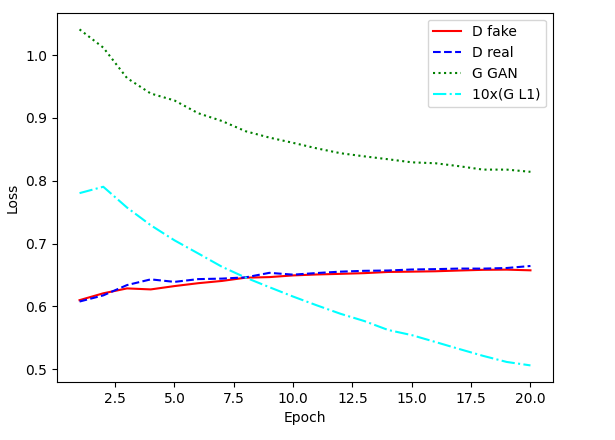
\includegraphics[width=15cm]{images/3_6.png}
\caption{Giá trị các thành phần mất mát của bộ phân biệt và bộ sinh qua từng epoch.}
\end{figure}

\noindent
Nhận thấy xu hướng của giá trị mất mát khi huấn luyện mô hình GAN là giá trị mất mát của bộ phân biệt tăng thì giá trị mất mát của bộ sinh sẽ giảm và cả hai dường như đều sẽ hội tụ về một giá trị. Lí giải điều này, khi bộ phân biệt đạt đến một ngưỡng thông minh nhất định, bộ sinh thì lại càng thông minh qua mỗi epoch, hiển nhiên sẽ đánh lừa được bộ phân biệt. Điều này là hợp lí với nguyên lí non-zero-sum-games. Ngoài ra, giá trị mất mát của bộ sinh theo chuẩn 1 cũng được giảm, tuy không đáng kể.

%%%%%%%%%%%%%%%%%%%%%%%%%%%%%%%%%
\section{Thử nghiệm và đánh giá mô hình}\label{testmodel}

\subsection{Mô hình GAN với bộ sinh đơn giản}\label{badexperiment}

Kết quả ở hình dưới là kết quả của mô hình được thử nghiệm với 5 bức ảnh ngẫu nhiên lấy từ tập COCO (không nằm trong tập huấn luyện). Khá không may mắn, kết quả không được như chúng ta mong đợi.

\begin{figure}[!h]
\captionsetup{width=0.8\textwidth}
\centering
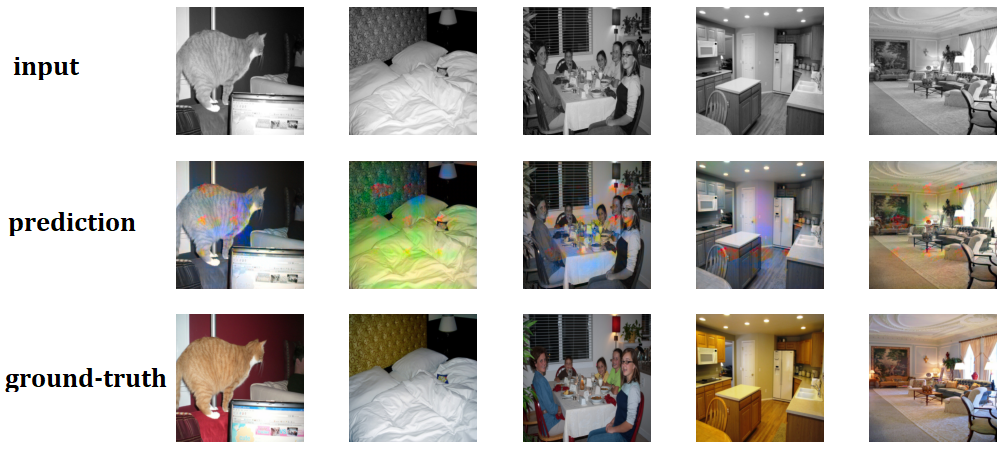
\includegraphics[width=15cm]{images/4_0.png}
\caption{Kết quả dự đoán của mô hình GAN với bộ sinh đơn giản sau epoch thứ 34 trên tập dữ liệu COCO.}
\label{fig:worseexperiment}
\end{figure}

\noindent
Nhìn chung, việc huấn luyện mô hình là khả thi khi mô hình cũng đã có thể tạo được màu cho một số điểm ảnh sau vài chục epoch. Nhưng như nêu ra phần \ref{transferlearning}, giới hạn về phần cứng cũng như là tập dữ liệu không đủ nhiều và tốt, để có thể huấn luyện được mô hình theo như mong đợi.\vspace{5pt}\\
Nhìn thêm ở một góc độ khác, việc huấn luyện một mạng GAN cũng không hề dễ dàng, khi GAN rất nhạy cảm với những thông số được cài đặt khi huấn luyện. Sau nhiều lần thử nghiệm thất bại, một trong số những kinh nghiệm rút ra là, trong hầu hết các mô hình GAN, ta nên khởi tạo các trọng số của mô hình và bias theo phân phối $\mathcal{N}\left(\mu, \sigma^2\right) = \mathcal{N}\left(0, 0.1\right)$ để quá trình huấn luyện nhanh hội tụ hơn. Dĩ nhiên không thể thiếu một điều kiện cần là một tập dữ liệu có chất lượng tốt.

\subsection{Mô hình GAN với bộ sinh có xương sống ResNet18}
\begin{figure}[!h]
\captionsetup{width=0.8\textwidth}
\centering
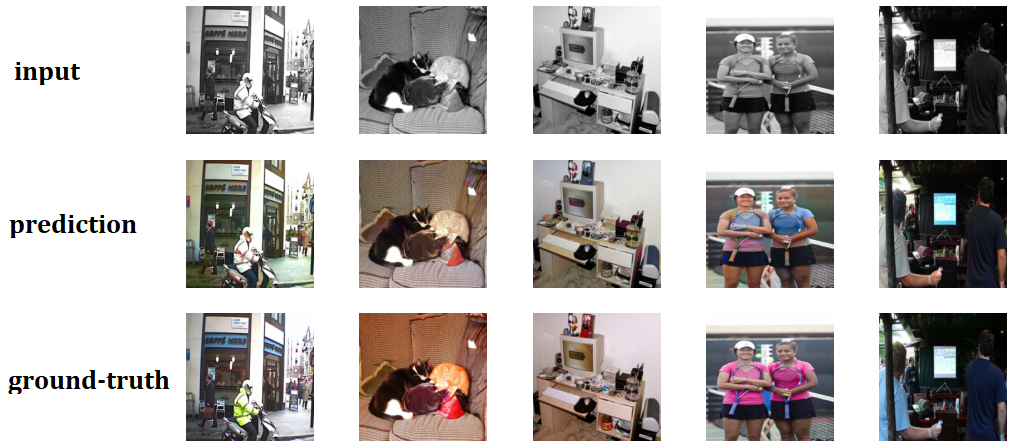
\includegraphics[width=15cm]{images/4_1.png}
\caption{Kết quả dự đoán của mô hình GAN với bộ sinh đơn giản có xương sống ResNet18 sau epoch thứ 15 trên tập dữ liệu COCO (không nằm trong tập huấn luyện).}
\label{fig:betterexperiment}
\end{figure}

\noindent
Kết quả ở hình \ref{fig:betterexperiment} dễ thấy đã cải thiện hơn hẳn so với kết quả ở hình \ref{fig:worseexperiment}. Màu tạo ra khi gắn với ảnh xám ít bị lem hay lộn xộn. Một vài đối tượng có màu khác với màu của ảnh gốc, ví dụ người lái xe ở ảnh phía trái ngoài cùng, nhưng vẫn hết sức hợp lí và tự nhiên.\vspace{5pt}\\
Một vài vùng ảnh, mô hình có vẻ như vẫn chưa thực sự chọn được màu phù hợp và rồi để màu gần giống với mức xám ban đầu. Để lí giải cho hạn chế này, có thể những vùng chưa có màu hợp lí là trong quá trình huấn luyện, mô hình chưa được học qua ảnh có đặc trưng, đối tượng tương tự.\vspace{5pt}

\begin{figure}[!h]
\captionsetup{width=0.8\textwidth}
\centering
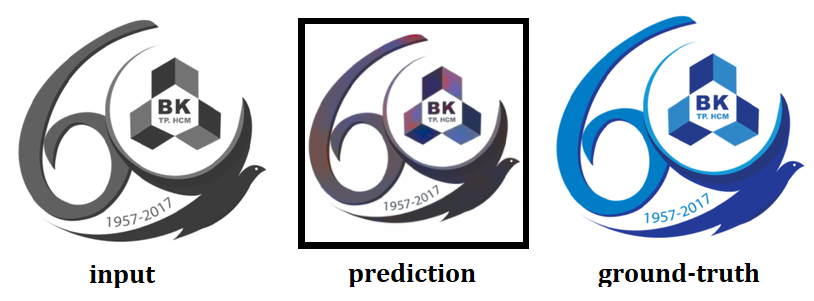
\includegraphics[width=15cm]{images/4_12.PNG}
\caption{Mô hình hoàn toàn bế tắc trước logo kỷ niệm 60 năm của trường ĐH Bách Khoa TP.HCM.}
\label{fig:failcolorlogo}
\end{figure}

\begin{figure}[!h]
\captionsetup{width=0.8\textwidth}
\centering
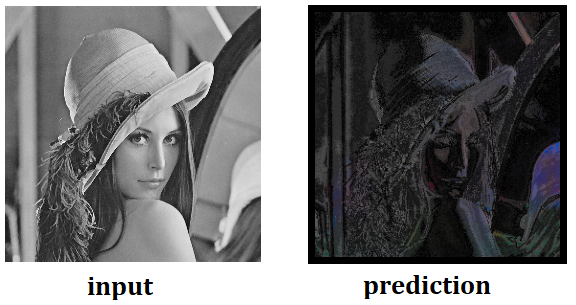
\includegraphics[width=12cm]{images/4_13.png}
\caption{Trường hợp đặc biệt khi mô hình làm việc tệ với ảnh có đặc trưng đơn giản.}
\label{fig:edgecase}
\end{figure}

\noindent
Điều trên dẫn đến một hạn chế khác nữa là đối với những ảnh không có đặc trưng rõ ràng, những đặc trưng mà chưa được đưa vào huấn luyện cho mô hình. Chẳng hạn ảnh chủ đề logo hình \ref{fig:failcolorlogo}, mô hình hoàn toàn không có khả năng tạo được màu phù hợp vì không hiểu được đặc trưng.\vspace{5pt}\\
Thêm một hạn chế khác là mô hình cũng chưa thực sự biết được những điểm ảnh nào sẽ cùng một đối tượng và cùng màu. Cụ thể như trong hình \ref{fig:betterexperiment}, ảnh hai cố gái cầm vợt tennis (thứ 2 từ phía bên phải), phần dưới của áo được chọn là màu hồng, còn phần trên của áo lại màu xanh. Nếu mô hình lựa cho phần áo màu hồng hay màu xanh thì đều chấp nhận được, nhưng mô hình lại chọn cách lựa hai phía của áo bởi hai màu khác nhau không đồng nhất.\vspace{5pt}\\
Riêng với hình \ref{fig:edgecase} thực sự là một kết quả bất ngờ, mà hiện tại vẫn chưa lí giải được tại sao mô hình cho kết quả không thực sự tốt. Việc mô hình không có khả năng làm việc với đặc trưng mặt người là không khả thi, khi ở phần \ref{compare} cũng có một ảnh mặt người tương tự và mô hình vẫn cho kết quả ổn. Đây là một trường hợp đặc biệt cần thêm nhiều tìm hiểu.

\subsection{So sánh bộ sinh có xương sống ResNet18 trước và sau khi huấn luyện đối nghịch}\label{compare}

Việc so sánh mô hình bộ sinh trước (bộ sinh đã được qua tiền huấn luyện đối lập) và sau khi huấn luyện đối nghịch cùng bộ phân biệt, sẽ cho ta thấy hiệu quả của mô hình GAN mang lại. Một số ảnh đen trắng được lựa chọn gồm các bối cảnh chân dung, phong cảnh, toà nhà cũng như những ảnh có nhiều đối tượng (chi tiết) để thử nghiệm.

\begin{figure}[!h]
\captionsetup{width=0.8\textwidth}
\centering
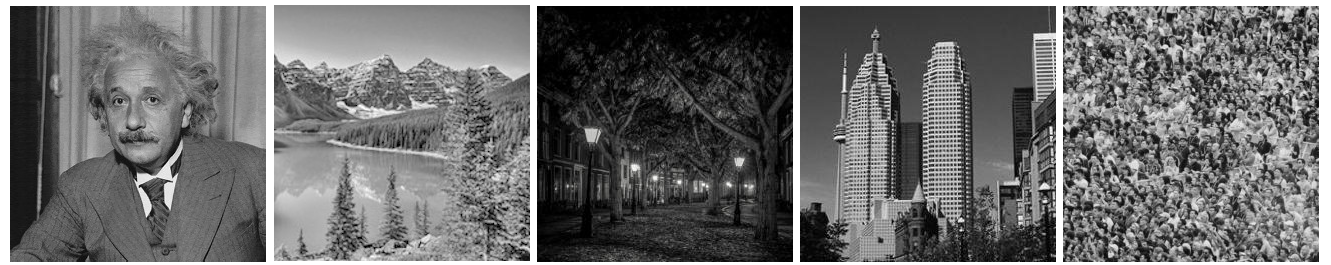
\includegraphics[width=15cm]{images/4_2.PNG}
\caption{Những tấm ảnh đen trắng được lựa chọn để so sánh sự khác biệt.}
\end{figure}

\noindent
Trước khi đưa cho mô hình thực hiện tạo màu, không khó để đoán được rằng hình ảnh đầu tiên (phía trái ngoài cùng) có ít chi tiết nhất nên khả năng cao sẽ có kết quả tốt nhất. Ngược lại, hình ảnh cuối cùng (phía phải ngoài cùng) có rất nhiều chi tiết nên kết quả cũng rất có thể không đạt được tốt như những tấm ảnh ít chi tiết. Và quả thật không ngoài dự đoán, kết quả đạt được khá đúng với những gì mong đợi.

\begin{figure}[!h]
\captionsetup{width=0.8\textwidth}
\centering
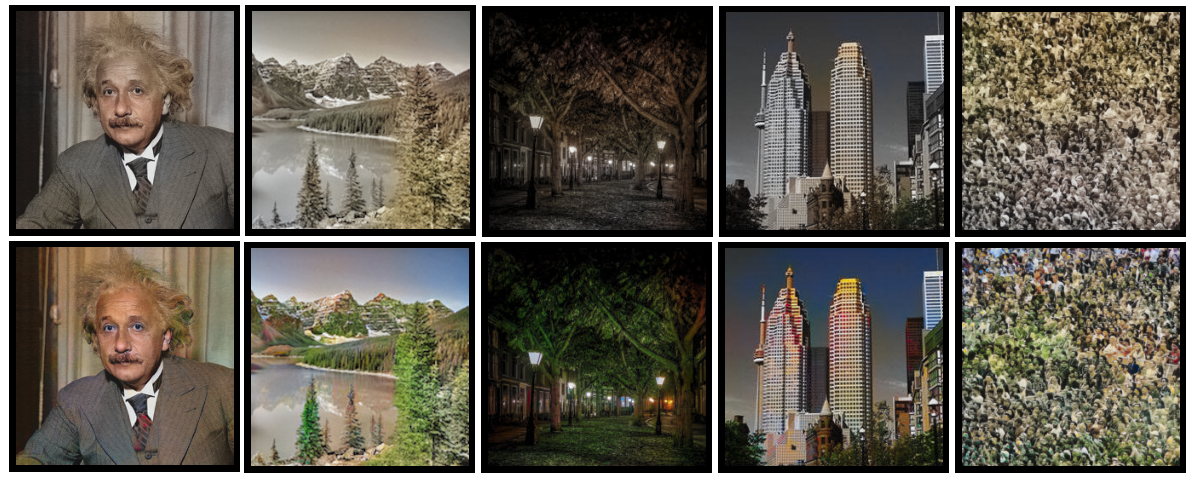
\includegraphics[width=15cm]{images/4_3.PNG}
\caption{Phía trên và dưới lần lượt là kết quả của bộ sinh trước và sau khi huấn luyện đối nghịch.}
\label{fig:comparesimpleandgan}
\end{figure}

\noindent
Ta có thể thấy trong hình \ref{fig:comparesimpleandgan} một điều là, mô hình sau khi được huấn luyện theo kiểu GAN cho kết quả có màu tươi sáng, chân thật hơn so với khi chưa được uốn nắn bởi bộ phân biệt. Kết quả đã cải thiện một cách rõ rệt, nên khó có thể nói là mô hình đối nghịch trong mạng GAN không có đóng góp mà chỉ do bộ sinh đã được huấn luyện thêm.\vspace{5pt}\\
Điểm yếu của việc áp dụng đơn giản hàm mất mát so sánh sai lệch giữa các điểm ảnh, bằng cách dùng chuẩn bậc 1 hoặc bậc 2 như thông thường, đối với bài toán tạo màu rất khó để có kết quả tốt, vì mô hình lúc này được khuyến khích để dùng màu xám. Điều này có thể lí giải là mô hình học được một quy tắc, khi không chắc chắn nên chọn màu gì, thì chọn một giá trị trung bình $(\mathbf{a^*}, \mathbf{b^*}) \approx (0, 0)$ là một cách an toàn nhất để có thể tối thiểu sai số, dẫn đến màu tạo ra có xu hướng không khác là mấy so với màu xám. Và dĩ nhiên màu trong cuộc sống của chúng ta rất nhiều màu sặc sỡ hơn màu xám dẫn, đến kết quả của mô hình trước khi đưa vào mạng GAN huấn luyện chưa đáp ứng mục tiêu hợp lí, chân thực đưa ra.

\subsection{Khảo sát đánh giá chất lượng mô hình}

\begin{figure}[!h]
\captionsetup{width=0.8\textwidth}
\centering
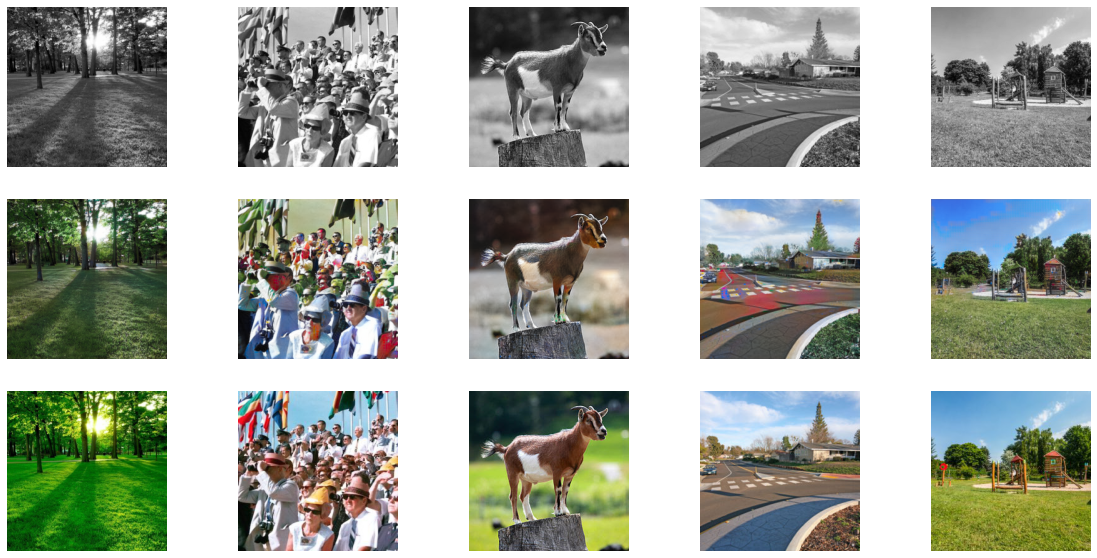
\includegraphics[width=15cm]{images/demo1.png}
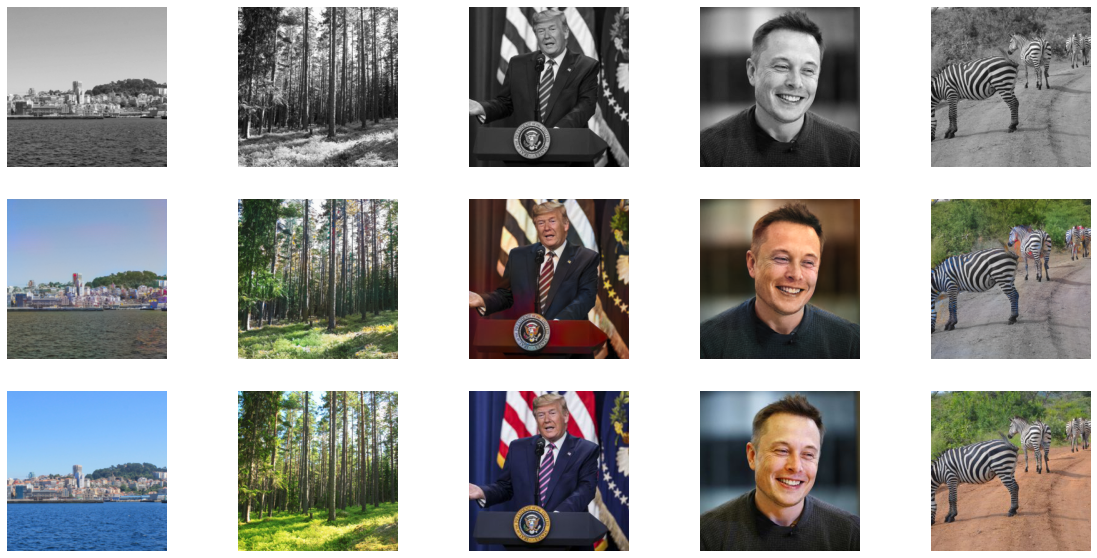
\includegraphics[width=15cm]{images/demo2.png}
\caption{Một số kết quả thử nghiệm khác. Các hàng lần lượt là ảnh xám, ánh sau khi tạo màu, ảnh gốc.}
\label{fig:moreresults}
\end{figure}

\begin{figure}[!h]
\captionsetup{width=0.8\textwidth}
\centering
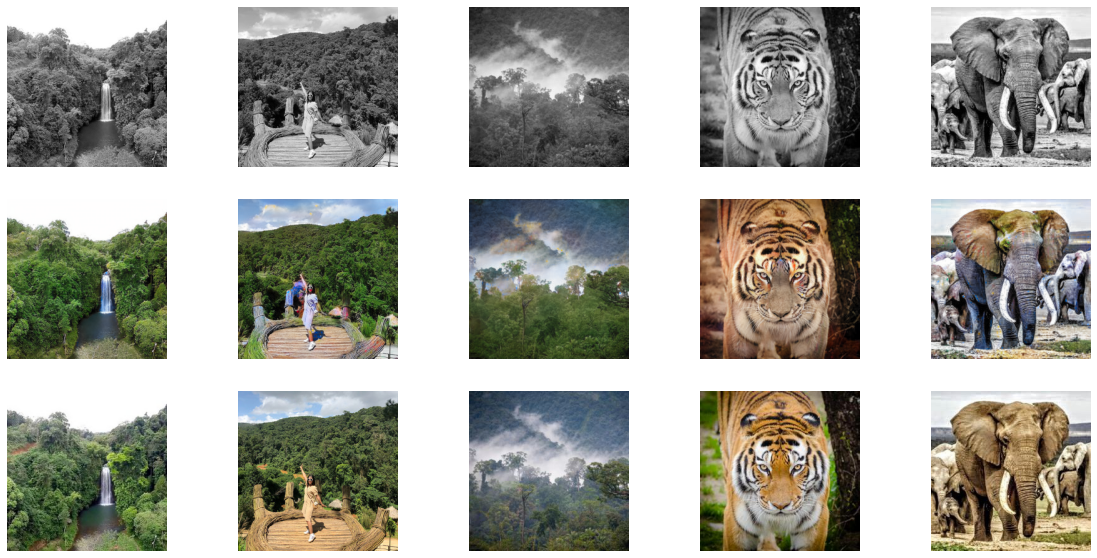
\includegraphics[width=15cm]{images/demo3.png}
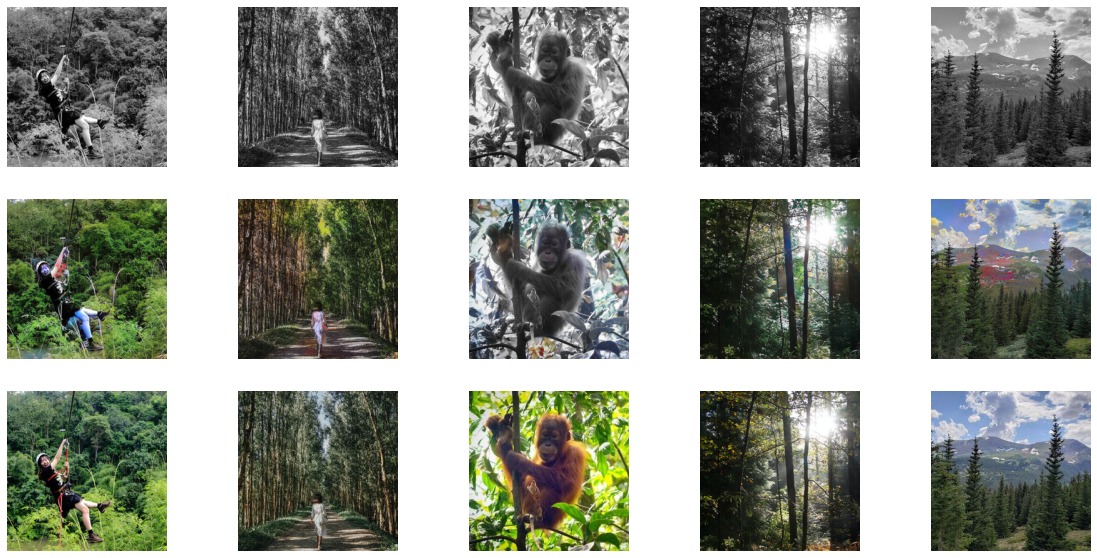
\includegraphics[width=15cm]{images/demo4.png}
\caption{Thêm Một vài kết quả thử nghiệm khác. Các hàng lần lượt là ảnh xám, ánh sau khi tạo màu, ảnh gốc.}
\label{fig:onemoreresults}
\end{figure}

\begin{figure}[!h]
\captionsetup{width=0.8\textwidth}
\centering

\includegraphics[width=12cm]{images/question.PNG}
\caption{Phần mô tả của bài đánh giá.}
\end{figure}

\noindent
Với nhiều bài toán liên quan về đồ hoạ, hình ảnh điển hình như bài toán tạo màu, một bài toán có nhiều lời giải thì một trong những bài kiểm tra tốt nhất là kiểm tra dưới góc độ của thị giác con người. Một cuộc khảo sát đã được tiến hành bởi sự giúp đỡ của 100 người, bao gồm những sinh viên thuộc cũng như không thuộc Đại học Quốc Gia và một số học sinh cấp trung học phổ thông. Bài kiểm tra đánh giá bao gồm 20 bức ảnh như trong \ref{fig:moreresults} và \ref{fig:onemoreresults}, được đánh số thứ tự từ trái sang phải, trên xuống dưới. Thang điểm đưa ra là từ 1 (rất giả) tới 5 (rất thật). Trong phần đánh giá, chỉ có ảnh sau khi tạo màu - ảnh ở hàng thứ hai để tránh thiên lệch khi đánh giá từ người tham gia.

\begin{figure}[!h]
\captionsetup{width=0.8\textwidth}
\centering
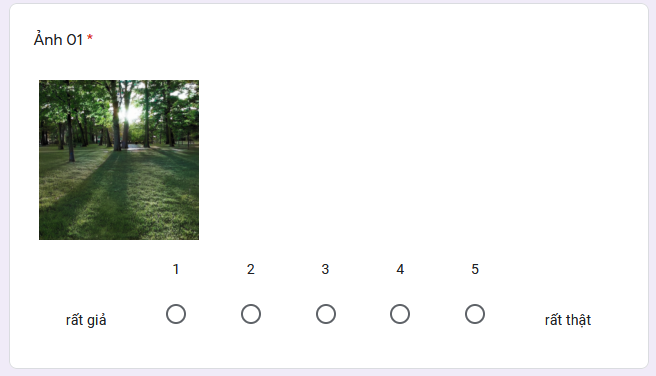
\includegraphics[width=12cm]{images/question2.PNG}
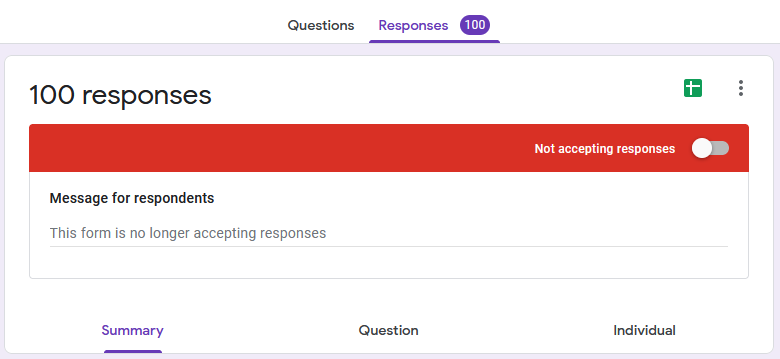
\includegraphics[width=12cm]{images/question3.PNG}
\caption[Phần câu hỏi và số lượng người tham gia cuộc khảo sát thực hiện thông qua Google Forms.]{Phần câu hỏi và số lượng người tham gia cuộc khảo sát thực hiện thông qua Google Forms\protect\footnotemark.}
\end{figure}
\footnotetext{Google Forms, \href{https://www.google.com/forms/about/}{https://www.google.com/forms/about/}}

\begin{table}[h!]
\centering
\begin{tabular}{|c|c|c|c|c|c|c|}
\hline
\diagbox[width=11em]{\textbf{Ảnh}}{\textbf{Thang điểm}}      & \textbf{1} & \textbf{2} & \textbf{3} & \textbf{4} & \textbf{5} & \textbf{Tổng} \\ \hline
\textbf{Ảnh 01}  & 2          & 11         & 29         & 36         & 22         & 100         \\ \hline
\textbf{Ảnh 02}  & 20         & 35         & 24         & 14         & 7          & 100         \\ \hline
\textbf{Ảnh 03}  & 1          & 11         & 21         & 34         & 33         & 100         \\ \hline
\textbf{Ảnh 04}  & 8          & 34         & 30         & 18         & 10         & 100         \\ \hline
\textbf{Ảnh 05}  & 2          & 7          & 18         & 34         & 39         & 100         \\ \hline
\textbf{Ảnh 06}  & 9          & 24         & 37         & 21         & 9          & 100         \\ \hline
\textbf{Ảnh 07}  & 1          & 12         & 15         & 34         & 38         & 100         \\ \hline
\textbf{Ảnh 08}  & 1          & 11         & 21         & 35         & 32         & 100         \\ \hline
\textbf{Ảnh 09}  & 1          & 10         & 21         & 30         & 38         & 100         \\ \hline
\textbf{Ảnh 10}  & 8          & 16         & 36         & 29         & 11         & 100         \\ \hline
\textbf{Ảnh 11}  & 4          & 8          & 19         & 33         & 36         & 100         \\ \hline
\textbf{Ảnh 12}  & 2          & 18         & 28         & 26         & 26         & 100         \\ \hline
\textbf{Ảnh 13}  & 7          & 18         & 22         & 34         & 19         & 100         \\ \hline
\textbf{Ảnh 14}  & 6          & 14         & 24         & 34         & 22         & 100         \\ \hline
\textbf{Ảnh 15}  & 13         & 27         & 40         & 12         & 8          & 100         \\ \hline
\textbf{Ảnh 16}  & 12         & 32         & 23         & 19         & 14         & 100         \\ \hline
\textbf{Ảnh 17}  & 14         & 26         & 30         & 18         & 12         & 100         \\ \hline
\textbf{Ảnh 18}  & 10         & 22         & 26         & 27         & 15         & 100         \\ \hline
\textbf{Ảnh 19}  & 3          & 8          & 23         & 29         & 37         & 100         \\ \hline
\textbf{Ảnh 20}  & 22         & 22         & 26         & 18         & 12         & 100         \\ \hline
\textbf{Tổng}  & 146         & 366         & 513         & 535         & 440      & 2000        \\ \hline
\end{tabular}
\caption{Kết quả bình chọn cho các ảnh.}
\label{tab:surveyresults}
\end{table}

\begin{table}[!h]
\centering
\begin{tabular}{c|c|c|c|c|c|}
\cline{2-6}
                                               & \textbf{Ảnh 01} & \textbf{Ảnh 02} & \textbf{Ảnh 03} & \textbf{Ảnh 04} & \textbf{Ảnh 05} \\ \hline
\multicolumn{1}{|c|}{\textbf{Điểm trung bình}} & 3.65            & \textbf{2.53}            & 3.87            & 2.88            & \textbf{4.01}            \\ \hline
\end{tabular}

\begin{tabular}{c|c|c|c|c|c|}
\cline{2-6}
                                               & \textbf{Ảnh 06} & \textbf{Ảnh 07} & \textbf{Ảnh 08} & \textbf{Ảnh 09} & \textbf{Ảnh 10} \\ \hline
\multicolumn{1}{|c|}{\textbf{Điểm trung bình}} & 2.97            & 3.96            & 3.86            & 3.94            & 3.19            \\ \hline
\end{tabular}

\begin{tabular}{c|c|c|c|c|c|}
\cline{2-6}
                                               & \textbf{Ảnh 11} & \textbf{Ảnh 12} & \textbf{Ảnh 13} & \textbf{Ảnh 14} & \textbf{Ảnh 15} \\ \hline
\multicolumn{1}{|c|}{\textbf{Điểm trung bình}} & 3.89            & 3.56             & 3.40            & 3.52            & 2.75            \\ \hline
\end{tabular}

\begin{tabular}{c|c|c|c|c|c|}
\cline{2-6}
                                               & \textbf{Ảnh 16} & \textbf{Ảnh 17} & \textbf{Ảnh 18} & \textbf{Ảnh 19} & \textbf{Ảnh 20} \\ \hline
\multicolumn{1}{|c|}{\textbf{Điểm trung bình}} & 2.91            & 2.88            & 3.15            & 3.89            & 2.76            \\ \hline
\end{tabular}
\caption{Điểm trung bình của các ảnh.}
\label{tab:statsurvey}
\end{table}

\noindent
Bảng \ref{tab:surveyresults} là kết quả bình chọn từ khảo sát 100 người. Không quá khó khăn để tính được điểm trung bình mà một tấm ảnh nhận được, bằng cách lấy tổng của số lượt bình chọn nhân với thang điểm tương ưng rồi chia cho tổng số bình chọn, ở đây là 100. Kết quả tính toán trên được cho ở bảng \ref{tab:statsurvey}.\vspace{5pt}\\
Trong những ảnh được bình chọn, ảnh có số điểm cao nhất là ảnh thứ \textbf{05} với \textbf{4.01} (mức 4/5) theo sau đó là những ảnh có số điểm 3.96 (07) và 3.94 (09) (xem hình \ref{fig:besttests}). Còn ảnh có số điểm thấp nhât là ảnh số \textbf{02} với \textbf{2.53} (mức 2--3/5), ngay phía trên là những ảnh có số điểm 2.75 (15) và 2.76 (20) (xem hình \ref{fig:worsttests}). Điểm trung bình của 20 bức ảnh khảo sát là \textbf{3.38} (mức 3) và có \textbf{11 (55\%)} ảnh có số điểm trung bình ở trên mức này.\vspace{5pt}\\
Một điều dễ nhận ra là những ảnh có cây cối, phong cảnh thiên nhiên sẽ là những ảnh có điểm khá cao, từ mức 3 tới mức 5. Và 2 trong số 3 bức ảnh đạt số điểm cao nhất cũng đều có đặc trưng như trên. Duy chỉ với ảnh 20, khi có phần tô lem nên đã bị đánh giá thấp đi nhiều, dẫu những phần còn lại có kết quả màu được tạo ra rất đẹp. Với những ảnh động vật thì kết quả không được khả quan như vậy, một trong số đó có kết quả gần tệ nhất là ảnh thứ tự 15. Chỉ riêng mỗi ảnh 03 có số điểm khá vượt trội so với những ảnh cùng đặc trưng. Với đặc trưng về con người, nếu không có quá nhiều chi tiết thì mô hình thể hiện khá tốt và cho số điểm rất cao (3.86 cho ảnh 08 và 3.94 cho ảnh 09). Nhưng với nhiều chi tiết thì mô hình lại không giữ được phong độ và cho kết quả cực kì tệ như ảnh 16 với số điểm 2.91 và ảnh số 02 với số điểm thấp nhất trong 20 bức ảnh khảo sát.

\begin{figure}[!h]
\captionsetup{width=0.8\textwidth}
\centering
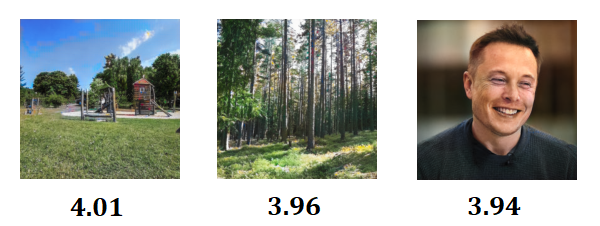
\includegraphics[width=12cm]{images/best.PNG}
\caption{Những ảnh có điểm trung bình cao nhất.}
\label{fig:besttests}
\end{figure}

\begin{figure}[!h]
\captionsetup{width=0.8\textwidth}
\centering
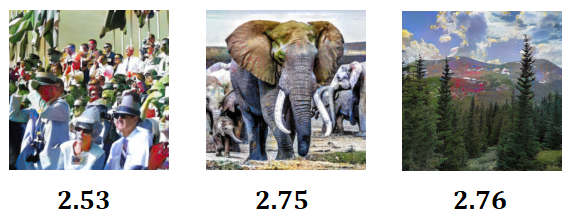
\includegraphics[width=12cm]{images/worst.PNG}
\caption{Những ảnh có điểm trung bình thấp nhất.}
\label{fig:worsttests}
\end{figure}

\noindent
Tuy số lượng mẫu khảo sát nhỏ với chỉ 20 bức ảnh (chưa đủ để làm tổng thể) và sự đa dạng không cao cũng như là số lượng người tham gia khảo sát không quá lớn, chỉ với 100 người, nhưng cũng phần nào đánh giá được chất lượng của mô hình. Nhìn chung, với số điểm trung bình 3.38 thì mô hình có thể xem ở mức \textbf{trung bình--khá}.

%%%%%%%%%%%%%%%%%%%%%%%%%%%%%%%%%
\section{Tổng kết}

\subsection{Kết luận}
Một phương pháp tạo màu cho ảnh xám đã được trình bày thông qua đồ án này. Phương pháp sử dụng khung mô hình một mạng đối nghịch tạo sinh có điều kiện - cGAN dùng bộ phân biệt Patch $70\times 70$, được huấn luyện theo kiểu đối nghịch kết hợp với một hàm mất mát chuẩn bậc 1 bằng tập dữ liệu 10,000 bức ảnh của COCO. Ánh xạ $\mathcal{G}:\mathbf{L^*} \rightarrow (\mathbf{a^*}, \mathbf{b^*})$ để tạo 2 kênh màu trong không gian màu \textbf{L*a*b*} chính là bộ sinh của mạng được thiết kế theo kiến trúc Unet có xương sống được học chuyển giao từ mô hình ResNet18 đã được tinh chỉnh.\vspace{5pt}\\
Chất lượng mô hình được đánh giá dựa qua một cuộc khảo sát thực tế, với sự tham gia giúp đỡ của 100 người. Bài khảo sát bao gồm 20 bức ảnh có màu tạo từ bộ sinh, theo thang điểm từ 1 (rất giả) tới 5 (rất thật). Kết quả nhận được là số điểm trung bình 3.38, trong đó số điểm cao nhất là 4.01 và thấp nhất là 2.53. Theo như mục tiêu được đề ra ở phần \ref{objective}, mô hình đã hoàn thành được ở mức trung bình--khá.

\subsection{Hướng cải thiện mô hình}

Mô hình vẫn chưa có kết quả tốt khi áp dụng với những ảnh có đặc trưng lạ, chưa được học trong quá trình huấn luyện. Để cải thiện trí tuệ mô hình, ta cần tìm thêm nhiều tập dữ liệu với các đối tượng, đặc trưng phong phú để huấn luyện thêm. Ngoài ra, sử dụng một xương sống được tinh chỉnh tốt hơn mạng ResNet18 hiện có, chẳng hạn ResNet34, ResNet50, ResNet101, hoặc một họ mạng khác như VGG hay Xception.\vspace{5pt}\\
Một cách tiếp cận khác để cải thiện mô hình, đó là huấn luyện nhiều bộ sinh, mỗi bộ sinh sẽ đảm nhiệm một nhóm đặc trưng nhất định. Như vậy chỉ cần cho bộ sinh học những ảnh liên quan đến chủ đề của mình. Bằng việc chuyên môn hoá chủ đề cho bộ sinh, ta không còn yêu cầu một bộ sinh có thể tạo màu tốt với mọi ảnh đầu vào. Thay vào đó, cho kết quả tốt hơn cả khi được đưa cho ảnh đúng chuyên môn. Quá trình huấn luyện cũng được đơn giản hơn do mô hình không phải học quá nhiều.\vspace{5pt}\\
Một số những đề xuất về việc sử dụng GAN để tạo màu có kết quả tốt có thêm tham khảo thêm như \cite{Nazeri_2018}, khi tác giả sử dụng mạng GAN tích chập sâu - DCGAN áp dụng với ảnh độ phân giải cao, tăng tốc độ và ổn định huấn luyện. Cao và các cộng sự của mình \cite{cao2017unsupervised} cũng sử dụng cGAN để tạo màu một cách đa dạng nhờ vào lấy mẫu nhiễu đầu vào nhiều lần. Một đột phá khác, Vitoria \cite{vitoria2020chromagan} nhận thấy rằng ta có tận dụng phân bố phân lớp trong quá trình huấn luyện cho mạng GAN, và đưa ra mô hình với cái tên là ChromaGAN.

\subsection{Hướng phát triển}
Đề tài có thể được áp dụng để làm những tác vụ liên quan đến phục chế màu cho ảnh xám, bị mất màu hoặc ảnh cũ xưa, thời chiến tranh. Giúp cho quá trình phục chế được tiết kiệm thời gian. Phối hợp với một ít tinh chỉnh bằng phương pháp thủ công, ta hoàn toàn có thể có những kết quả phục chế đẹp đẽ và tiết kiệm được rất nhiều thời gian.\vspace{5pt}\\
Không chỉ dừng lại ở hình ảnh, ta cũng có thể áp dụng mô hình để phục chế màu cho các video, vì bản chất một video là sự kết hợp từ nhiều khung hình ghép lại. Trong thư mục đồ án, phần \texttt{test\_results} có một kết quả thử nghiệm của mô hình qua việc phục chế màu một đoạn nhỏ về phóng sự về chiến tranh ở Việt Nam.

\begin{figure}[!h]
\centering
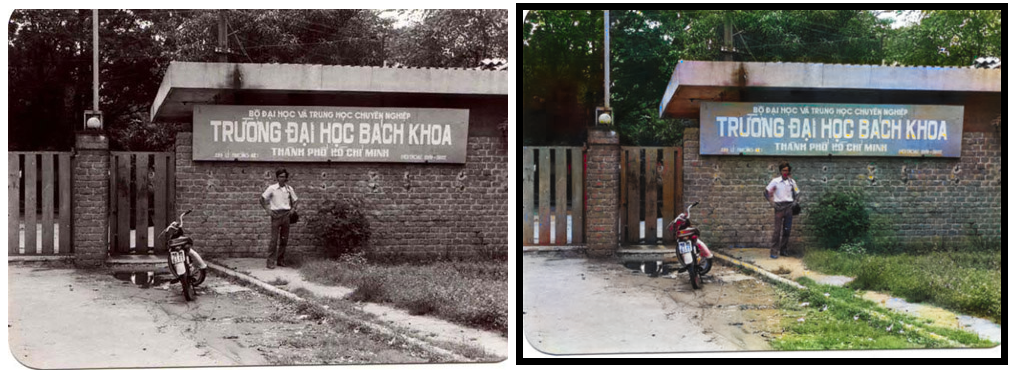
\includegraphics[width=15cm]{images/5_1.PNG}
\caption{Ảnh Trường ĐH Bách Khoa TP.HCM ngày xưa (trái) và sau khi tô màu (phải)}
\label{fig:bkhcmold}
\end{figure}

\newpage
\vspace*{\fill}
{\centering \textit{Trang này được cố ý để trống.}\par}
\vspace{\fill}
\newpage

%%%%%%%%%%%%%%%%%%%%%%%%%%%%%%%%%
\section{Phục lục - Ảnh màu}

\begin{figure}[!h]
\captionsetup{width=0.8\textwidth}
\centering
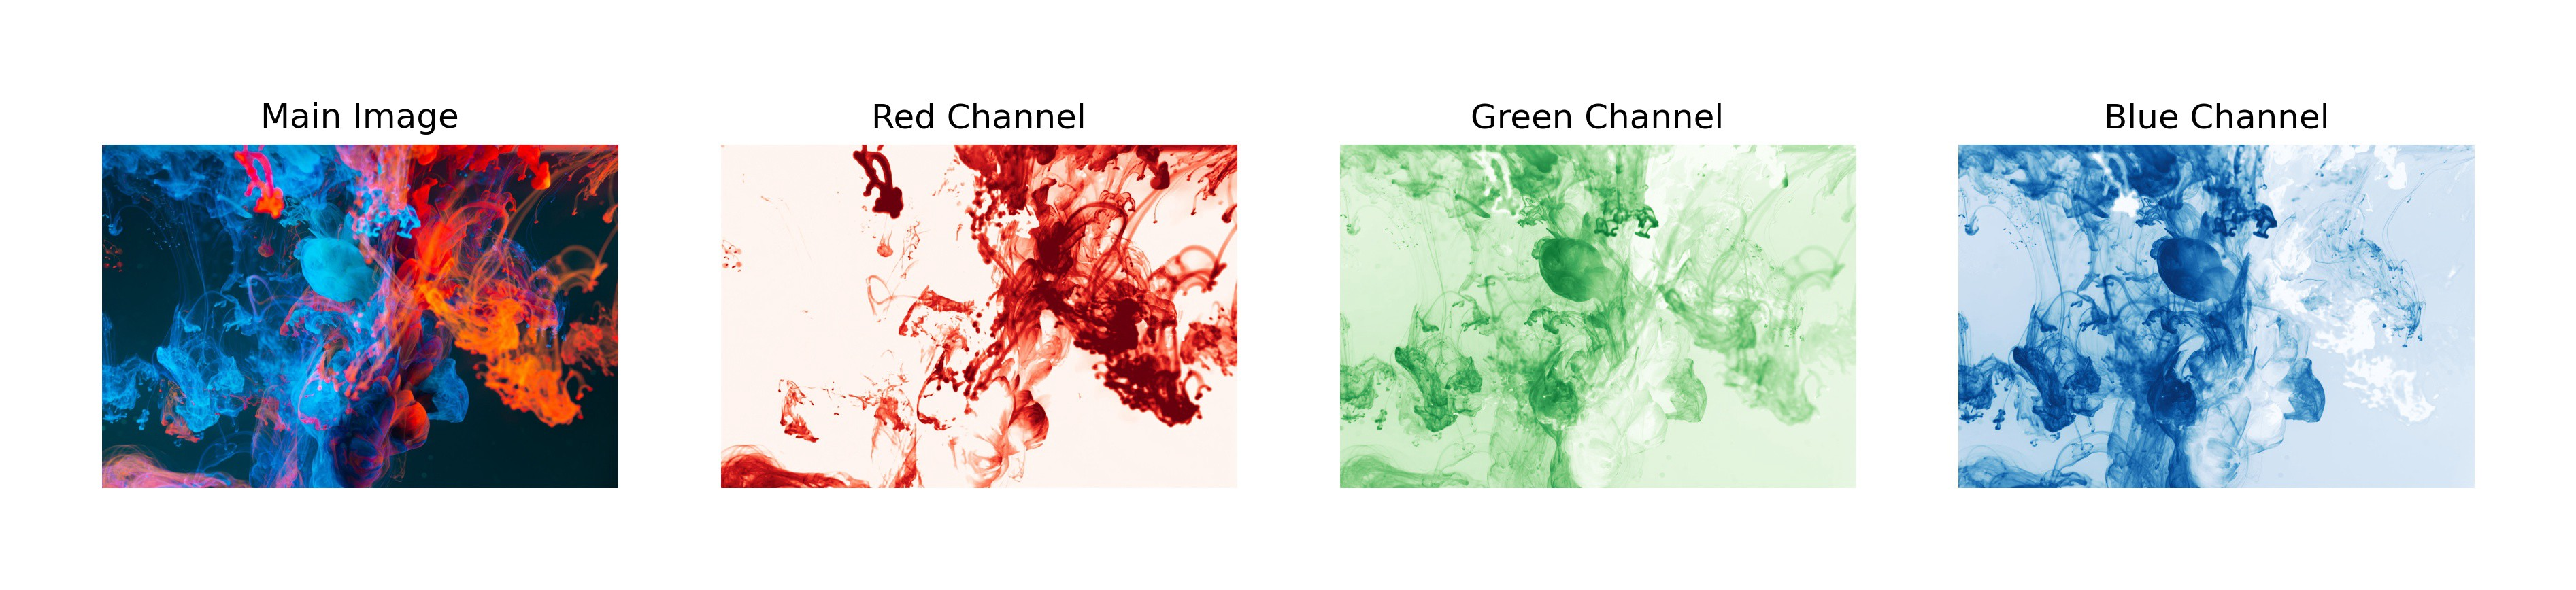
\includegraphics[width=16cm]{images/2_1.jpeg}
% \caption[]{Các kênh màu đỏ, lục và lam được tách ra riêng biệt \cite{moeincolorization2020}.}
\caption*{Hình \ref{fig:inspectrgb}: Các kênh màu đỏ, lục và lam được tách ra riêng biệt \cite{moeincolorization2020}.}
\end{figure}

\begin{figure}[!h]
\captionsetup{width=0.8\textwidth}
\centering
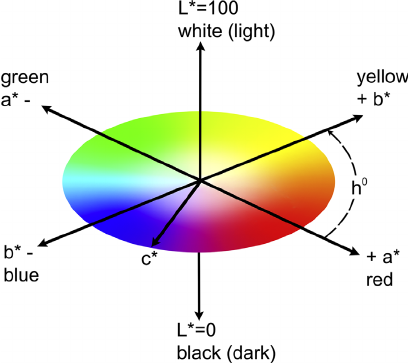
\includegraphics[width=8cm]{images/2_2.png}
\caption*{Hình \ref{fig:labspace}: Không gian màu Lab.}
\end{figure}

\begin{figure}[!h]
\captionsetup{width=0.8\textwidth}
\centering
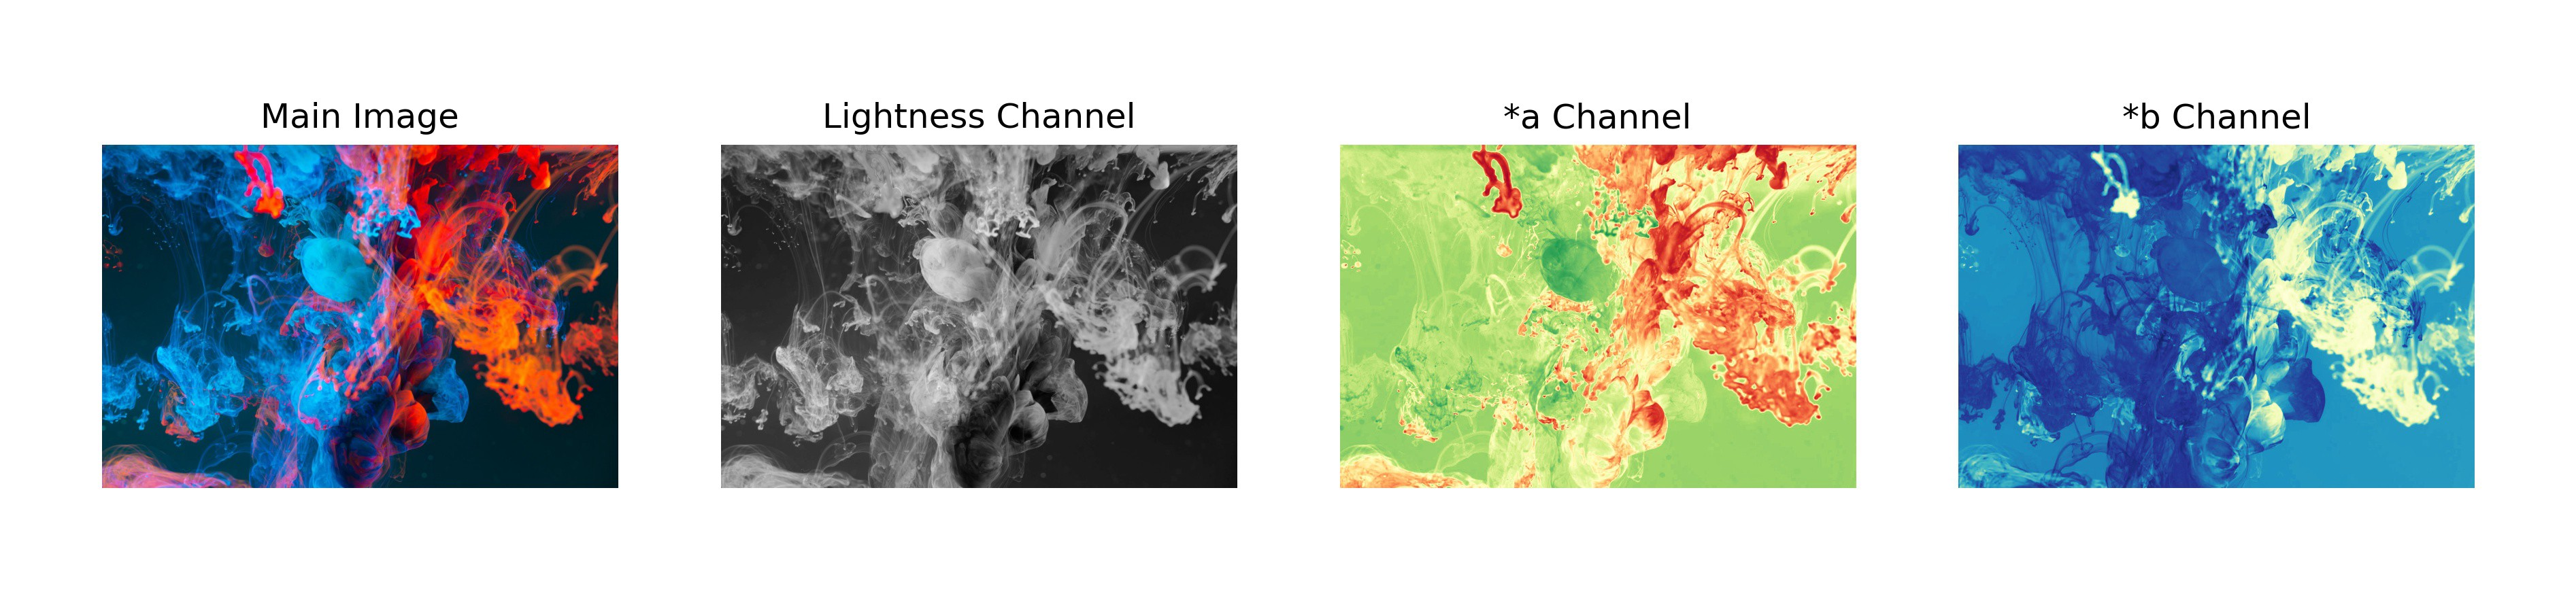
\includegraphics[width=16cm]{images/2_3.jpeg}
\caption*{Hình \ref{fig:inspectlab}: Các giá trị \textbf{L}, \textbf{a} và \textbf{b} được tách ra riêng biệt \cite{moeincolorization2020}.}
\end{figure}

\begin{figure}[!h]
\captionsetup{width=0.8\textwidth}
\centering
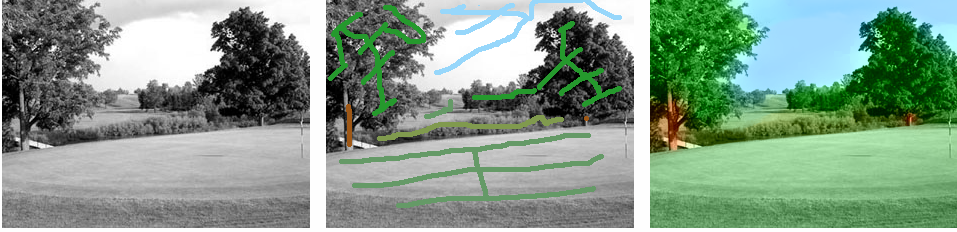
\includegraphics[width=15cm]{images/2_4.png}
\caption*{Hình \ref{fig:scribblemethod}: Mô tả ý tưởng thuật toán đánh dấu vài điểm ảnh \cite{trungcolorization2018}.}
\end{figure}

\begin{figure}[!h]
\captionsetup{width=0.8\textwidth}
\centering
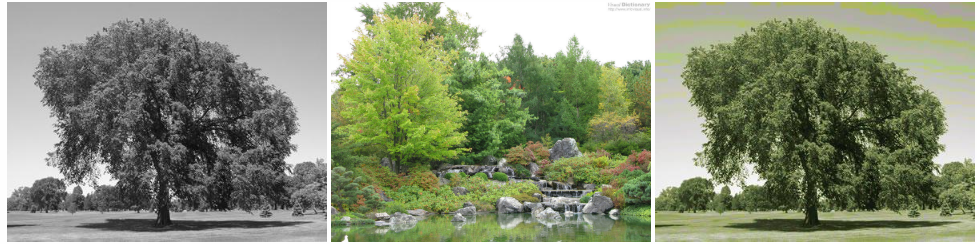
\includegraphics[width=15cm]{images/2_5.png}
\caption*{Hình \ref{fig:examplarmethod}: Mô tả ý tưởng thuật toán ảnh có bố cục tương tự \cite{trungcolorization2018}.}
\end{figure}

\begin{figure}[!h]
\captionsetup{width=0.8\textwidth}
\centering
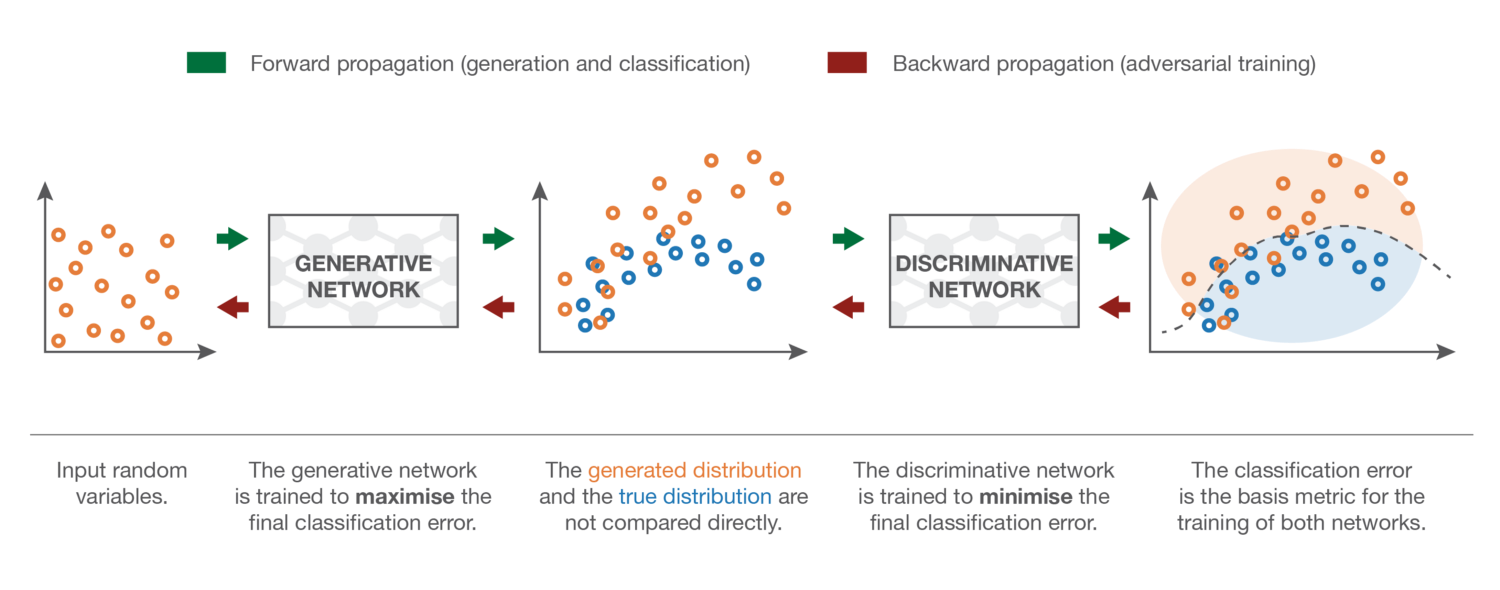
\includegraphics[width=16.5cm]{images/2_72.png}
\caption*{Hình \ref{fig:forandbackgan}: Mô phỏng quá trình huấn luyện mạng GAN \cite{josephgan2019}.}
\end{figure}

\begin{figure}[!h]
\captionsetup{width=0.8\textwidth}
\centering
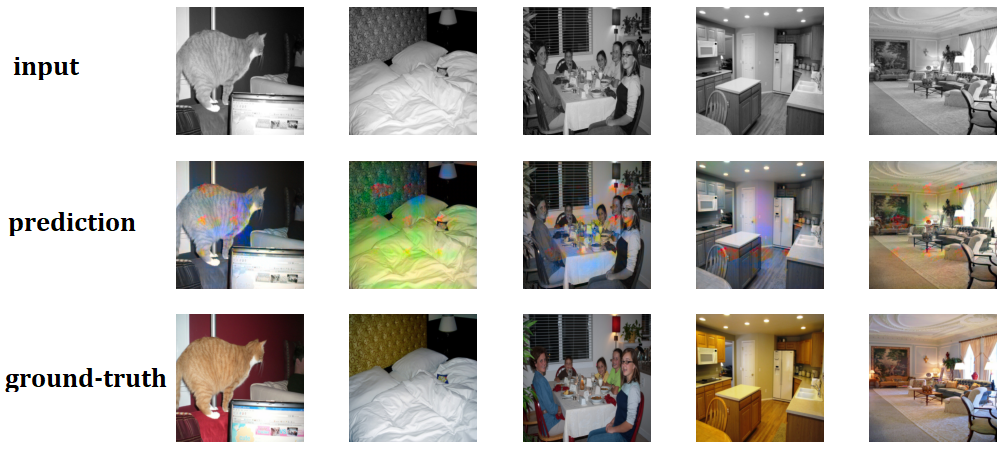
\includegraphics[width=15cm]{images/4_0.png}
\caption*{Hình \ref{fig:worseexperiment}: Kết quả dự đoán của mô hình GAN với bộ sinh đơn giản sau epoch thứ 34 trên tập dữ liệu COCO.}
\end{figure}

\begin{figure}[!h]
\captionsetup{width=0.8\textwidth}
\centering
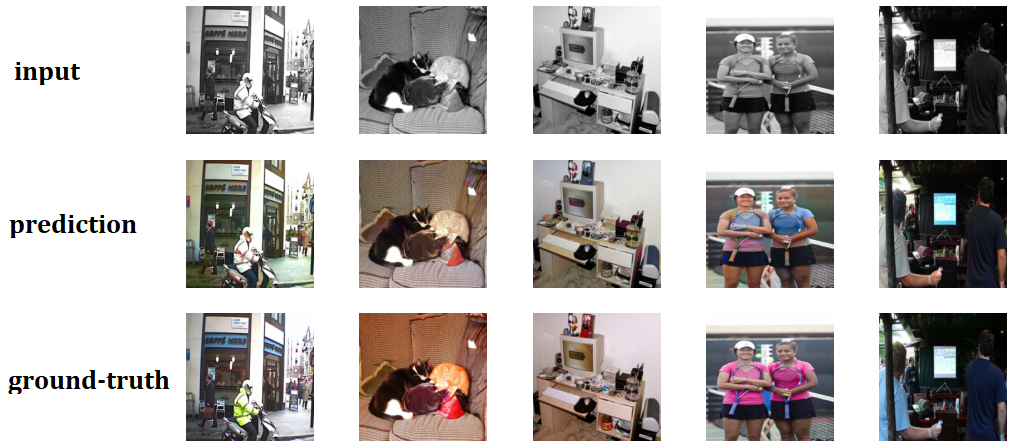
\includegraphics[width=15cm]{images/4_1.png}
\caption*{Hình \ref{fig:betterexperiment}: Kết quả dự đoán của mô hình GAN với bộ sinh đơn giản có xương sống ResNet18 sau epoch thứ 15 trên tập dữ liệu COCO (không nằm trong tập huấn luyện).}
\end{figure}

\begin{figure}[!h]
\captionsetup{width=0.8\textwidth}
\centering
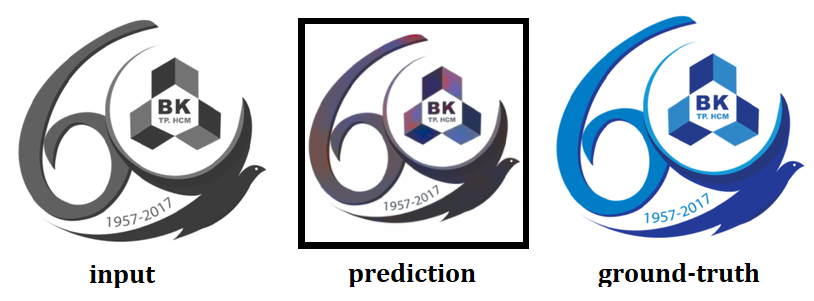
\includegraphics[width=15cm]{images/4_12.PNG}
\caption*{Hình \ref{fig:failcolorlogo}: Mô hình hoàn toàn bế tắc trước logo kỷ niệm 60 năm của trường ĐH Bách Khoa TP.HCM.}
\end{figure}

\begin{figure}[!h]
\captionsetup{width=0.8\textwidth}
\centering
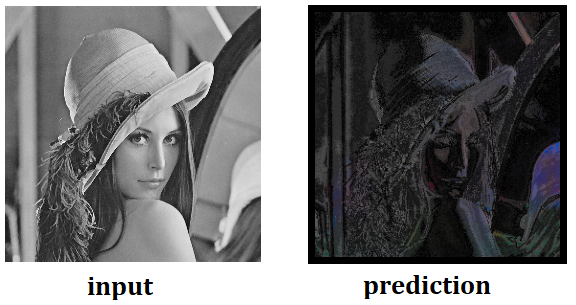
\includegraphics[width=12cm]{images/4_13.png}
\caption*{Hình \ref{fig:edgecase}: Trường hợp đặc biệt khi mô hình làm việc tệ với ảnh có đặc trưng đơn giản.}
\end{figure}

\begin{figure}[!h]
\captionsetup{width=0.8\textwidth}
\centering
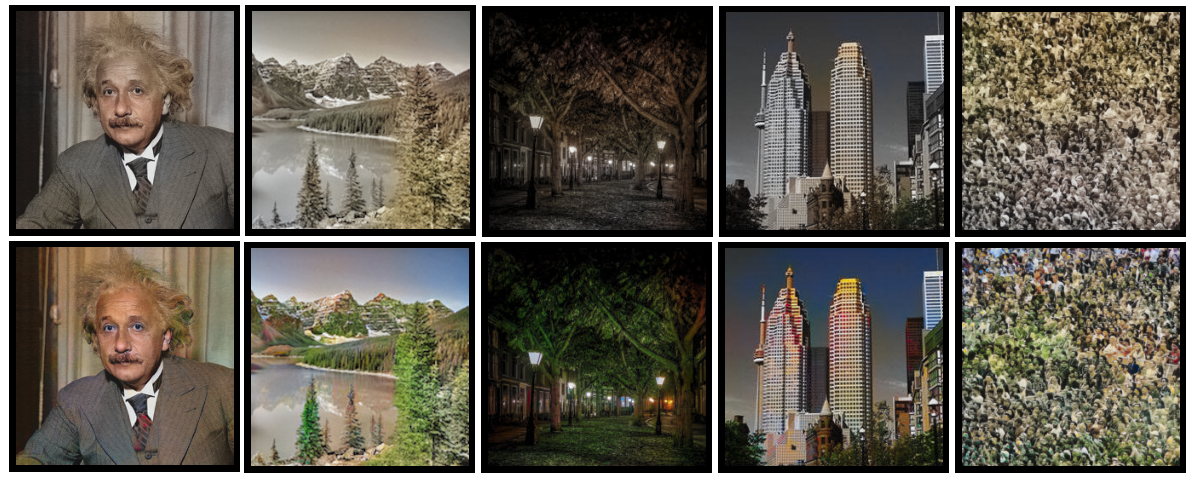
\includegraphics[width=15cm]{images/4_3.PNG}
\caption*{Hình \ref{fig:comparesimpleandgan}: Phía trên và dưới lần lượt là kết quả của bộ sinh trước và sau khi huấn luyện đối nghịch.}
\end{figure}

\begin{figure}[!h]
\captionsetup{width=0.8\textwidth}
\centering
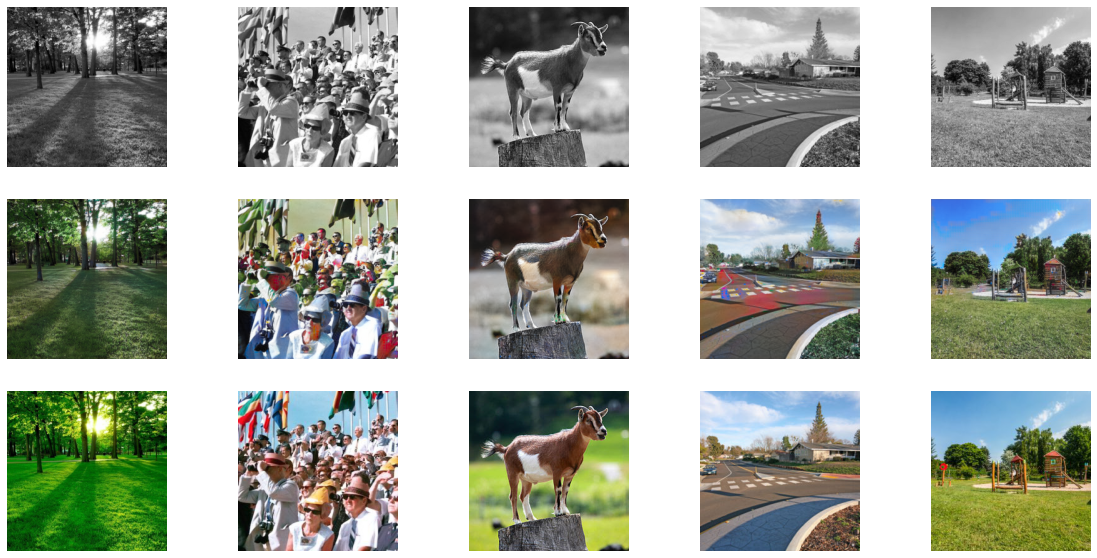
\includegraphics[width=15cm]{images/demo1.png}
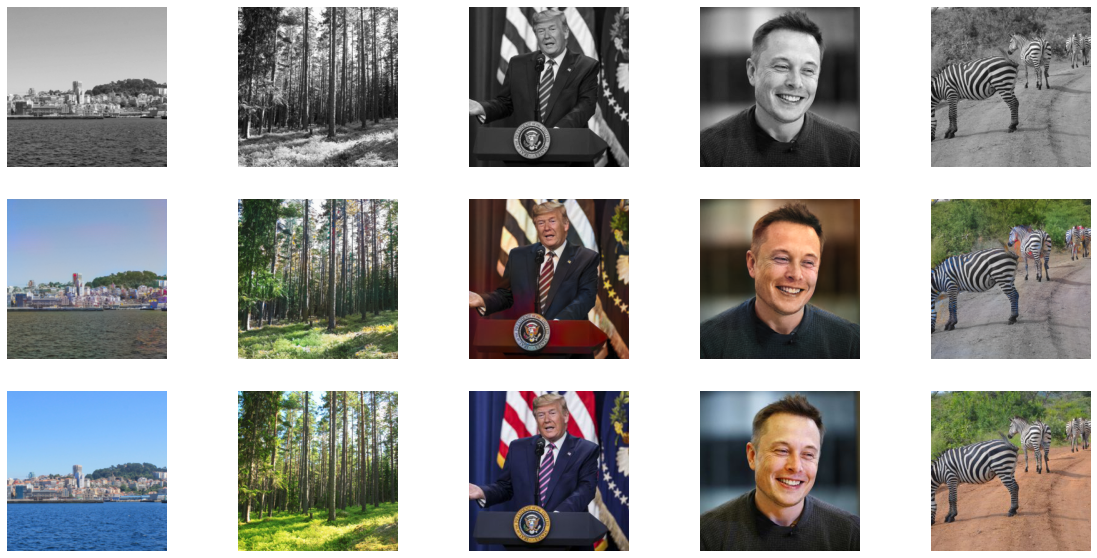
\includegraphics[width=15cm]{images/demo2.png}
\caption*{Hình \ref{fig:moreresults}: Một số kết quả thử nghiệm khác. Các hàng lần lượt là ảnh xám, ánh sau khi tạo màu, ảnh gốc.}
\end{figure}

\begin{figure}[!h]
\captionsetup{width=0.8\textwidth}
\centering
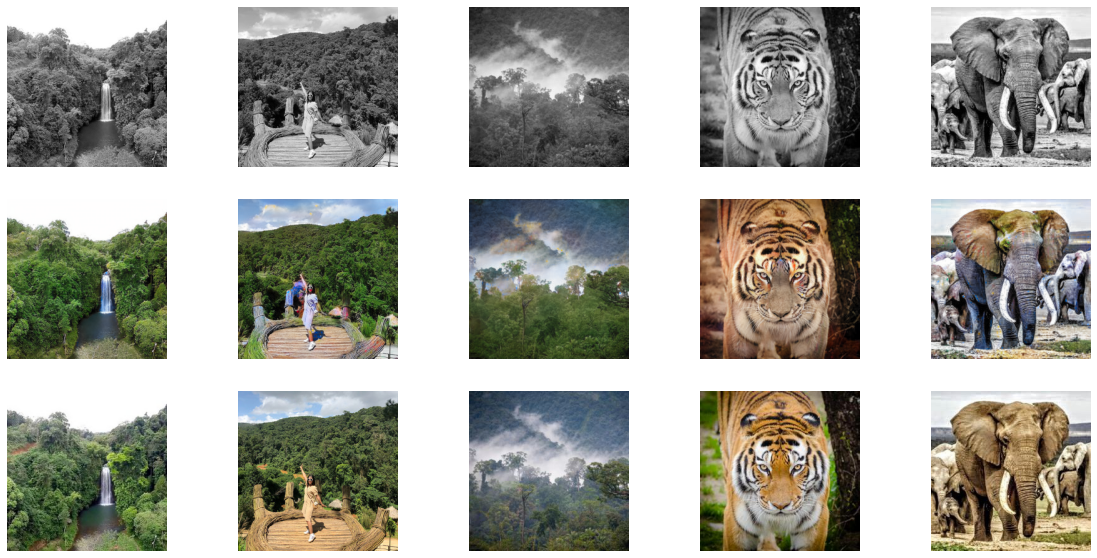
\includegraphics[width=15cm]{images/demo3.png}
\includegraphics[width=15cm]{images/demo4.png}
\caption*{Hình \ref{fig:onemoreresults}: Thêm Một vài kết quả thử nghiệm khác. Các hàng lần lượt là ảnh xám, ánh sau khi tạo màu, ảnh gốc.}
\end{figure}

\begin{figure}[!h]
\centering
\includegraphics[width=15cm]{images/5_1.PNG}
\caption*{Hình \ref{fig:bkhcmold}: Ảnh Trường ĐH Bách Khoa TP.HCM ngày xưa (trái) và sau khi tô màu (phải)}
\end{figure}

\clearpage

\renewcommand{\refname}{Tài liệu tham khảo}
%%%%%%%%%%%%%%%%%%%%%%%%%%%%%%%%%

\printbibliography

\end{document}